\chapter{矩阵与变换}

\begin{introduction}
  \item 从方程组到矩阵
  \item 从线性变换到矩阵
  \item 矩阵的运算
  \item 矩阵的性质
\end{introduction}

参考资料:
\begin{enumerate}
    \item \href{https://github.com/afshinea/stanford-cs-229-machine-learning/blob/master/zh/refresher-algebra-calculus.pdf}{Machine Learning cheatsheets for Stanford's CS 229 - VIP Refresher: Linear Algebra and Calculus};
    \item \href{https://math.mit.edu/~gs/linearalgebra/ila5/indexila5.html}{Introduction to Linear Algebra, Fifth Edition (2016)};
    \item 高等代数(第四版),高等教育出版;
    \item 高中数学人教A版选修4-2:矩阵与变换.
\end{enumerate}

%%%%%%%%%%%%%%%%%%%%%%%%%%%%%%%%%%%%%%%%%%%
\section{从方程组到矩阵}
\label{sec:origin_of_matrix}

\begin{note}
本节旨在帮助学生了解矩阵产生的原因,它源于人们在解方程组时对简洁表达的需求。
\end{note}

\subsection{二元一次方程组}
\label{subsec:二元一次方程组}

让我们首先回顾一下二元一次方程组的基本概念。一个二元一次方程组由两个含有两个变量的一次方程组成。一般形式如下:

\begin{equation}
\left\{
\begin{array}{l}
ax_1 + bx_2 = c\\
dx_1 + ex_2 = f
\end{array}
\right.
\label{eq:二元一次方程组通式}
\end{equation}

其中,\(x_1\) 和 \(x_2\) 是我们要找的未知数,而 \(a\)、\(b\)、\(c\)、\(d\)、\(e\) 和 \(f\) 是已知的常数。

要解这样的方程组,我们通常会使用以下两种方法之一:
\begin{enumerate}
    \item \textbf{代数方法}:这种方法包括“代入法”和“消元法”。
    \begin{enumerate}
        \item 在代入法中,我们从一个方程中解出一个变量的表达式,然后将其代入另一个方程;
        \item 在消元法中,我们通过加减两个方程来消除一个变量,从而找到另一个变量的值。
    \end{enumerate}
    \item \textbf{图形方法}:在这种方法中,我们将每个方程视为二维空间中的一条直线。方程组的解就是这两条直线的交点。
\end{enumerate}


下面,我们使用\textbf{消元法}来解以下二元一次方程组:

\begin{equation}
    \left\{
        \begin{array}{l}
        2x_1 + 3x_2 = 5\\
        4x_1 + 5x_2 = 7
        \end{array}
        \right.
\label{eq:二元一次方程组示例}
\end{equation}

我们的目标是找到满足这两个方程的\(x_1\)和\(x_2\)的值。我们可以通过以下步骤来实现这一目标:

\begin{enumerate}
    \item 首先,我们可以使用第一个方程来消去第二个方程中的\(x_1\)。为此,我们可以将第一个方程的两边都乘以2,得到新的方程:
    \[
    4x_1 + 6x_2 = 10
    \]
    \item 接着,我们将新得到的方程从第二个方程中减去,从而消去\(x_1\):
    \[
    4x_1 + 5x_2 - (4x_1 + 6x_2) = 7 - 10
    \]
    这将给我们一个只包含\(x_2\)的方程:
    \[
    -x_2 = -3
    \]
    从中我们可以找到\(x_2\)的值:
    \[
    x_2 = 3
    \]
    \item 事实上,\(x_2 = 3\)可以看成一个方程,我们可以使用它来消去第一个方程中的\(x_2\):
    \[
    (2x_1 + 3x_2) + (-3) \cdot x_2 = 5 + (-3) \cdot 3
    \]
    这将给我们:
    \[
    2x_1 = 5 - 9
    \]
    从中我们可以找到\(x_1\)的值:
    \[
    2x_1 = -4
    \]
    \[
    x_1 = -2
    \]
\end{enumerate}

所以,该方程组的解是:
\[
x_1 = -2, \quad x_2 = 3
\]


在下一节中,我们将介绍如何使用高斯消元法和矩阵来更简洁地表达求解过程。

\vspace{0.3cm}

\noindent 使用Python可以很轻松地解出方程组\ref{eq:二元一次方程组示例}。

\lstinputlisting[language=python]{scripts/code-1-1-4.py}

\begin{note}
    用方程$u$减去方程$v$指:用方程$u$的左边减去方程$v$的左边,用方程$u$的右边减去方程$v$的右边。
\end{note}

\subsection{系数矩阵和增广矩阵}
\label{subsec:系数矩阵和增广矩阵}

考虑二元一次方程组(\ref{eq:二元一次方程组示例})。
我们将方程组中方程的所有系数按照它们在整理好的方程中的位置取出来写成如式\ref{eq:系数矩阵示例}的一张数表。
有了这张数表我们就可以更加简洁地表达方程组中未知数的系数,
因此我们将其称为方程组的\textcolor{third}{\bf 系数矩阵},我们将其记为大写字母$A$。
由于矩阵$A$的尺寸是$2\times 2$,因此我们称其为$2\times 2$矩阵,或者$2$阶(方形)矩阵。

\begin{equation}
  A = \left(\begin{array}{ll}
2 & 3 \\
4 & 5
\end{array}\right)
\label{eq:系数矩阵示例}
\end{equation}

如果我们在系数矩阵右边增加一列$c$,用于记录方程的右端项(right hand side, RHS),则方程组(\ref{eq:二元一次方程组示例})可以写作$Ax=\boldsymbol{b}$。我们用一根竖线隔开表示系数的数表和表示右端项的数列,得到的整个新数表称为方程组\ref{eq:二元一次方程组示例}的\textcolor{third}{\bf 增广矩阵},如式\ref{eq:增广矩阵示例}所示:
\begin{equation}
    [A \mid c]=\left(\begin{array}{cc|c}
2 & 3 & 5 \\
4 & 5 & 7
\end{array}\right)
\label{eq:增广矩阵示例}
\end{equation}

下面,我们对增广矩阵实施第\ref{subsec:二元一次方程组}节中所使用的消元法,从而达到解方程的目的:

\begin{enumerate}
    \item 首先,我们用第一行的系数来将第二行的系数化为$0$,具体操作如下:
    \begin{enumerate}
        \item 用第二行的第一个系数$4$除以第一行的第一个系数$2$,得到商数$2$;
        \item 将第一行整体乘以此商数($2$),得到$(4,6,10)$;
        \item 再用第二行减去第一行,则第二行的第一个元素变为$0$。这时增广矩阵变为:
        \begin{equation}
            \left(\begin{array}{cc|c}
        2 & 3 & 5 \\
        0 & -1 & -3
        \end{array}\right)
        \label{eq:行阶梯形矩阵}
        \end{equation}
        \item 在第二行两边乘以$-1$
    \end{enumerate}
    \item 现在用第二行中$x_2$的系数来将第一行中$x_2$的系数化为$0$,具体操作如下:
    \begin{enumerate}
        \item 用第一行的第二个系数$3$除以第二行的第二个系数$1$,得到商数$3$;
        \item 将第二行整体乘以此商数($3$),得到$(0,3,9)$;
        \item 再用第一行减去第二行,则第一行的第二个元素变为$0$。这时增广矩阵变为:
        \[
        \left(\begin{array}{cc|c}
        2 & 0 & -4 \\
        0 & 1 & 3
        \end{array}\right)
        \]
        \item 在第一行两边乘以$\frac{1}{2}$,得到增广矩阵:
        \begin{equation}
            \left(\begin{array}{cc|c}
        1 & 0 & -2 \\
        0 & 1 & 3
        \end{array}\right)
        \label{eq:简化行阶梯形矩阵}
        \end{equation}
    \end{enumerate}
\end{enumerate}

该式还原为方程组为

\[
\left\{
\begin{array}{l}
1 \cdot x_1 + 0 \cdot x_2 = -2\\
0 \cdot x_1 + 1\cdot x_2 = 3
\end{array}
\right.
\]


最终得到$x_1=-2$,$x_2=3$,这就是原方程组的解。

矩阵提供了一种组织方程组系数和常数项的方式,通过矩阵运算可以方便地求解方程组。这启发了矩阵理论的产生和发展。


\subsection{高斯-若尔当消元法}
\label{subsec:高斯-若尔当消元法}

回顾我们在第\ref{subsec:系数矩阵和增广矩阵}节中的操作,我们在增广矩阵上进行消元法时,仅仅使用了两种操作:
\begin{itemize}
    \item 把某行乘以一非零常数;
    \item 把第 $i$ 行加上第 $j$ 行的 $k$ 倍;
\end{itemize}

可见这些操作都是对矩阵的“行”进行的,因此我们称它们为\textcolor{third}{\bf 行变换}。

注意到,在进行消元法的过程中,我们得到的增广矩阵\ref{eq:行阶梯形矩阵}的非零元素看起来像是一个“倒过来的楼梯”,其第一行左起第一个非零元下方都是零,第二行左起第一个非零元在第一行左起第一个非零元的右侧,我们称这样的矩阵是\textcolor{third}{\bf 行阶梯形矩阵}。

\begin{definition}[行阶梯形矩阵]
    如果一个矩阵满足下面的条件,我们称其为{\bf 行阶梯形矩阵}(Row Echelon Form):
    \begin{enumerate}
        \item 所有仅包含零的行都位于矩阵的最底部;
        \item 在每一个非零行中,最左边的非零元素(称主元)总是出现在上一行主元的右侧;
        \item *包含非零元素的行中,首个非零元素必须为$1$.
    \end{enumerate}
    其中第三个条件是可选的,不同文献中有不同的定义方式,不必纠结。
\end{definition}

事实上,得到增广矩阵\ref{eq:行阶梯形矩阵}后,我们已经不再需要继续消元了。从第二行我们可以很容易的得到$-x_2=-3$,从而解出$x_2=3$。从第一行我们得到方程$2x_1+3x_2=5$,这时候我们使用\textbf{回代法},将$x_2=3$代到方程$2x_1+3x_2=5$中得到$2x_1+3\cdot 3=5$,从而解出$x_1=-2$。

一般地,我们称\textcolor{second}{“先通过行变换将矩阵化为行阶梯矩阵,然后直接通过回代法找到方程组的解”}这样的解方程的方法为\textcolor{third}{\bf 高斯消元法}。可以证明,任何矩阵都可以通过高斯消元法转换为简化行阶梯形形式

此外,当消元法进行到尾声时,我们得到的增广矩阵\ref{eq:简化行阶梯形矩阵}非常有特点,其每一行的第一个非零元素全是$1$,且这些行的第一个元素$1$所在列的其余元素全为零,我们称这样的矩阵是\textcolor{third}{\bf 简化行阶梯形矩阵}。显然,根据简化行阶梯形矩阵我们很容易得到方程组的解。

\begin{definition}[简化行阶梯形]
    如果一个矩阵满足下面的条件,我们称其为{\bf 简化行阶梯形}(Reduced Row Echelon Form, RREF):
\begin{enumerate}
    \item 所有零行都位于矩阵的底部;
    \item 在每一个非零行中,第一个非零元素(称主元)总是出现在上一行主元的右侧;
    \item 每一个非零行的主元都是$1$;
    \item \textcolor{red}{一个主元所在的列的其他元素都是$0$}。
\end{enumerate}

简化行阶梯形和行阶梯形矩阵的主要区别在于最后一条。

\end{definition}

一般地,我们称\textcolor{second}{“先通过行变换将矩阵化为行阶梯矩阵,然后进一步做行变换,将其化为简化行阶梯形矩阵进而直接\textbf{读出}方程组的解”}这样的解方程的方法为\textcolor{third}{\bf 高斯-若尔当消元法}。可以证明,任何矩阵都可以通过高斯-若尔当消元法转换为简化行阶梯形形式。高斯-若尔当消元法实际上是高斯消元法的一个扩展。需要指出的是,虽然我们这里借助高斯消元法行变换来引入行变换,但是行变换并不是只能在增广矩阵上进行,因为行变换是一种矩阵变形的方法,并不限定于某种特殊的矩阵。

\subsection{矩阵的行列式}
\label{subsec:矩阵的行列式}

\begin{note}
    行列式来自于数学家们在求解方程组时发现的一个可以用来简化表达,并判断方程组是否有解的记号。
\end{note}

\vspace*{0.3cm}

考虑二元一次    方程组(\ref{eq:二元一次方程组通式}),我们使用高斯-若尔当消元法求出该方程的解。
\begin{equation*}
\left[
\begin{array}{cc|c}
a & b & c \\
d & e & f
\end{array}
\right]
\xrightarrow{}
    \left[
    \begin{array}{cc|c}
1 & \frac{b}{a} & \frac{c}{a} \\
0 & e - \frac{bd}{a} & f - \frac{cd}{a}
\end{array}
\right]
\xrightarrow{}
\left[
\begin{array}{cc|c}
1 & 0 & \frac{ce - bf}{ae - bd} \\
0 & 1 & \frac{af - cd}{ae - bd}
\end{array}
\right]
\end{equation*}

如果我们定义$D=ae - bd, D_1=ce-bf, D_2=af - cd$,我们可以将原方程的结果表示为:
\begin{equation}
x_1 = \frac{D_1}{D},\quad x_2 = \frac{D_2}{D}
\end{equation}

这个结果称为二元一次方程组的\textcolor{third}{\bf 克莱姆法则}(Cramer's Rule)。其中$D$称为矩阵
$
\begin{bmatrix}
a & b \\
d & e
\end{bmatrix}
$
的行列式,记作
\begin{equation}
D = \operatorname*{det} \left(
    \begin{bmatrix}
        a & b \\
        d & e
        \end{bmatrix}
\right) = 
\left|
    \begin{array}{cc}
    a & b \\
    d & e
    \end{array}
\right|
= ae - bd
\end{equation}

同理有,

\begin{equation}
    D_1 = \operatorname*{det} \left(
        \begin{bmatrix}
            c & b \\
            f & e
            \end{bmatrix}
    \right) = 
    \left|
        \begin{array}{cc}
            c & b \\
            f & e
        \end{array}
    \right| = ce-bf, \quad
    D_2 = \operatorname*{det} \left(
        \begin{bmatrix}
            a & c \\
            d & f
            \end{bmatrix}
    \right) = 
    \left|
        \begin{array}{cc}
        a & c \\
        d & f
        \end{array}
    \right| = af - cd
\end{equation}

考虑一个特殊的方程组
\begin{equation}
    \left\{
        \begin{array}{l}
        x_1 + x_2 = 5\\
        x_1 + x_2 = 7
        \end{array}
        \right.
\end{equation}

显然,该方程组无解,其中$D=0$。可见,凡是系数矩阵的行列式$D=0$的二元一次方程组都是无解的。


一般地,考虑任意$n$元一次方程组(矩阵表示):
\begin{equation}
    A x=c
\label{eq:一般方程组的矩阵形式}
\end{equation}

其中的 $A$ 是一个 $n \times n$ 的方阵, 而向量 $x=\left(x_1, x_2, \cdots x_n\right)^T$和$c=\left(c_1, c_2, \cdots c_n\right)^T$ 均为长度为 $n$ 的列向量。 

克莱姆法则说明: 如果 $\operatorname{det} A \neq 0$ ,那么方程(\ref{eq:一般方程组的矩阵形式})有解$x=\left(x_1, x_2, \cdots x_n\right)^T$,其中

$$
x_i=\frac{\operatorname{det}\left(A_i\right)}{\operatorname{det}(A)}
$$

当中 $x_i$ 是列向量 $x$ 的第 $i$ 行,$A_i$ 是用列向量 $c$ 取代 $A$ 的第 $i$ 列后得到的矩阵。

注意到,我们仅定义了二阶方阵的行列式,那么对于任意一个$n \times n$ 的方阵$A$,如何计算$\operatorname{det}(A)$呢?具体的计算方式依赖于行列式的三种定义:
\begin{itemize}
    \item 用排列和逆序数定义(国内大多数教材上都用这种定义);
    \item 利用代数余子式和按第一行展开进行归纳定义;
    \item 利用其几何意义(有向面积在一般的欧几里得空间中的推广)进行定义.
\end{itemize}

本讲义中我们希望大家按照几何意义来理解行列式,我们可以将其视作在一定的线性变换(比如旋转、缩放)下,形状的面积(在二维空间)或体积(在三维空间)的缩放因子。想象你有一张纸,上面画了一个单位正方形。这个正方形的边长都是1,所以它的面积也是1。现在,如果我们用一个矩阵来表示一个变换,比如把这个正方形拉长或者压扁,或者同时进行拉长和压扁的组合,那么变换后的图形可能就不再是正方形,而是一个矩形或任意四边形。

行列式的值,就是这个变换后的图形的面积与原来单位正方形面积的比值。如果行列式的值大于1,那么面积被放大了;如果行列式的值小于1但大于0,那么面积被缩小了;如果行列式的值是负数,这意味着除了面积或体积的缩放,还发生了一个“翻转”操作,比如在二维空间中,图形被沿原点镜像反转了。

在三维空间中,这个解释同样适用,但这次是关于体积的缩放而不仅仅是面积。如果你有一个单位立方体,通过一个矩阵表示的线性变换后,立方体可能会变成任意的平行六面体。这时候,行列式的绝对值就告诉我们变换后的平行六面体的体积是如何相对于单位立方体的体积进行缩放的。\textcolor{red}{三阶行列式计算比较好记,可以顺手补充一下。}

简而言之,行列式给我们提供了一个数值,这个数值说明了在一个线性变换下,形状的尺寸如何改变:面积或体积是如何扩大或缩小的,以及是否发生了方向的翻转。高阶行列式的具体计算比较复杂,我们可以使用\texttt{NumPy}代劳,我们只需要理解其意义即可。

%%%%%%%%%%%%%%%%%%%%%%%%%%%%%%%%%%%%%%%%%%%
\section{通用符号}

\begin{note}
    本节最重要却最容易忽略的一点:数学文本中,如无特殊说明,则一般认为向量都是\textcolor{red}{列向量}。
\end{note}

\subsection{向量}
我们记$\boldsymbol{x}\in \mathbb{R}^n$为一个 $n$ 维的向量, 其中 $x_i \in \mathbb{R}$ 是第 $i$ 维的元素:
$$
\boldsymbol{x}=\left(\begin{array}{c}
x_1 \\
x_2 \\
\vdots \\
x_n
\end{array}\right) \in \mathbb{R}^n
$$

\subsection{矩阵}
我们记 $A \in \mathbb{R}^{m \times n}$ 为一个 $m$ 行 $n$ 列的矩阵, 其中 $a_{i, j} \in \mathbb{R}$ 是第 $i$ 行 $j$ 列的元素:
$$
A=\left(\begin{array}{ccc}
a_{1,1} & \cdots & a_{1, n} \\
\vdots & & \vdots \\
a_{m, 1} & \cdots & a_{m, n}
\end{array}\right) \in \mathbb{R}^{m \times n}
$$

注意: 如上定义的向量 $\boldsymbol{x}$ 可以被看做是一个 $n \times 1$ 的矩阵,常被称为一个列向量。


\subsection{单位矩阵}

单位矩阵 $I \in \mathbb{R}^{n \times n}$ 是一个方形矩阵(或简称为方阵),其对角线的元素上均为 1, 其余位置均为 0 。
$$
I=\left(\begin{array}{cccc}
1 & 0 & \cdots & 0 \\
0 & \ddots & \ddots & \vdots \\
\vdots & \ddots & \ddots & 0 \\
0 & \cdots & 0 & 1
\end{array}\right)
$$

% 注: 对所有矩阵 $A \in \mathbb{R}^{n \times n}$, 我们有 $A \times I=I \times A=A$ (\textcolor{red}{讲完矩阵乘法回来解释该式})。


\subsection{对角阵}

对角阵 $D \in \mathbb{R}^{n \times n}$ 是一个方阵其对角线上元素均是非零值, 其余位置均为 0 。
$$
D=\left(\begin{array}{cccc}
d_1 & 0 & \cdots & 0 \\
0 & \ddots & \ddots & \vdots \\
\vdots & \ddots & \ddots & 0 \\
0 & \cdots & 0 & d_n
\end{array}\right)
$$

注: 我们记 $D$ 为 $\operatorname{diag}\left(d_1, \ldots, d_n\right)$ 。

\subsection{三角矩阵}

三角矩阵(triangular matrix)因其非零系数的排列呈三角形状而得名。

一个如下形状的方形矩阵:
$$
\mathbf{L}=\left[\begin{array}{ccccc}
l_{1,1} & & \ldots & & 0 \\
l_{2,1} & l_{2,2} & & (0) & \\
l_{3,1} & l_{3,2} & \ddots & & \vdots \\
\vdots & \vdots & \ddots & \ddots & \\
l_{n, 1} & l_{n, 2} & \ldots & l_{n, n-1} & l_{n, n}
\end{array}\right]
$$

被称为下三角矩阵;同样的, 一个如下形状的方形矩阵:

$$
\mathbf{U}=\left[\begin{array}{ccccc}
u_{1,1} & u_{1,2} & u_{1,3} & \ldots & u_{1, n} \\
& u_{2,2} & u_{2,3} & \ldots & u_{2, n} \\
\vdots & & \ddots & \ddots & \vdots \\
& (0) & & \ddots & u_{n-1, n} \\
0 & & \ldots & & u_{n, n}
\end{array}\right]
$$

被称为上三角矩阵。
\textcolor{red}{值得注意的是,三角矩阵一定是方阵。}

%%%%%%%%%%%%%%%%%%%%%%%%%%%%%%%%%%%%%%%%%%%
\section{矩阵与线性变换}
%参考高中数学选修4-2中的例子
\label{sec:矩阵与线性变换}

\begin{note}
    矩阵与线性变换通过一次方程组建立联系。事实上,在直角坐标系 $O x y$ 中, 所有满足“线性”性质的几何变换都具有形式
$$
\left\{\begin{array}{l}
x^{\prime}=a x+b y, \\
y^{\prime}=c x+d y,
\end{array}\right.
$$

其中 $a, b, c, d$ 均为常数. 该变换可以由二阶矩阵 $\left(\begin{array}{ll}a & b \\ c & d\end{array}\right)$ 完全确定.
\end{note}

本节将以矩阵为工具, 研究一些几何变换, 并以平面图形的变换为背景, 讨论二阶矩阵的乘法及性质, 用变换的观点理解解二元一次方程组的意义, 初步展示矩阵应用的广泛性。

\subsection{几种特殊几何变换}
\label{subsec:几种特殊几何变换}

\subsubsection{恒等变换}
\label{subsubsec:恒等变换}

相传,在古希腊德尔斐的阿波罗神庙中,刻有“认识你自己”这句箴言,它鼓励人们深入探索自我,以实现更深层次的理解和个人成长。这句古老的箴言也在数学中找到了回音。我们在定义任何数学对象之间的关系时,一定要先思考这种关系在对象和它自身之间是否是存在的。比如,实数相等和不相等的关系,就需要建立在每个实数都和它自身相等的基础上。

我们在研究平面上的几何变换时也有类似的概念,这就是本节要介绍的\textcolor{third}{\bf 恒等变换},它是一种将一个对象变换为其自身的变换。这意味着,在这种变换下,对象保持不变。

 在直角坐标系 $O x y$ 内, 恒等变换将每个点都映射为它自身(即相当于没有发生变化). 设点 $P(x, y)$ 经过恒等变换后变成点 $P^{\prime}\left(x^{\prime}, y^{\prime}\right)$,则 $x^{\prime}, y^{\prime}$ 与 $x, y$ 有如下关系:

\begin{equation}
\left\{\begin{array}{l}
x^{\prime}=x, \\
y^{\prime}=y .
\end{array}\right.
\label{eq:恒等变换的表达式}
\end{equation}

我们将式(\ref{eq:恒等变换的表达式})称为恒等变换的表达式。对式\ref{eq:恒等变换的表达式}进行简单改写,如式\ref{eq:恒等变换的方程}所示:

\begin{equation}
\left\{\begin{array}{l}
x^{\prime}=x + 0\cdot y, \\
y^{\prime}= 0\cdot x + y .
\end{array}\right.
\label{eq:恒等变换的方程}
\end{equation}

故其系数矩阵为:

\begin{equation}
\left(\begin{array}{rr}
1  & 0 \\
0  & 1
\end{array}\right)
\label{eq:恒等变换矩阵}
\end{equation}

可见,恒等变换的表达式的系数矩阵正好是一个单位矩阵,因此我们将单位矩阵称为恒等变换的\textcolor{third}{变换矩阵}。单位矩阵也唯一确定了一种变换,即恒等变换。因此,在讨论数学问题时,你常常能听到人们指着单位矩阵说:“这是一个恒等变换”。

\subsubsection{旋转变换}
\label{subsubsec:旋转变换}

在第\ref{subsubsec:恒等变换}节中,我们已经得到了平面上的点到它自身的变换,现在我们可以开始研究平面上的点到其他与它不同的点的变换了。

如图 \ref{fig:旋转变换} 所示, 在直角坐标系 $O x y$ 内, 每个点都绕原点 $O$ 按逆时针方向旋转 $180^{\circ}$. 设点 $P(x, y)$ 经过旋转后变成点 $P^{\prime}\left(x^{\prime}, y^{\prime}\right)$,则 $x^{\prime}, y^{\prime}$ 与 $x, y$ 有如下关系:

\begin{equation}
\left\{\begin{array}{l}
x^{\prime}=-x, \\
y^{\prime}=-y .
\end{array}\right.
\label{eq:旋转变换的表达式}
\end{equation}

我们将式(\ref{eq:旋转变换的表达式})称为旋转角为 $180^{\circ}$ 的\textcolor{third}{\bf 旋转变换}的表达式, 它建立了平面内的每个点 $P$ 到其对应点 $P^{\prime}$ 的对应关系, 我们称 $P^{\prime}$ 是 $P$ 在这个旋转变换作用下的像.

\begin{figure}[h]
\centering
\begin{tikzpicture}[scale=1.5]
    % 绘制坐标轴
    \draw[->] (-1.5,0) -- (1.5,0) node[right] {$x$};
    \draw[->] (0,-1.5) -- (0,1.5) node[above] {$y$};

    % 绘制原点O
    \coordinate (O) at (0,0);
    \fill (O) circle (0pt) node[anchor=north east] {$O$};
    
    % 绘制旋转前的点P
    \coordinate (P) at (1,1);
    \fill (P) circle (2pt) node[anchor=south west] {$P(x, y)$};
    
    % 绘制旋转后的点P'
    \coordinate (P') at (-1,-1);
    \fill (P') circle (2pt) node[anchor=north east] {$P'(x', y')$};
    
    % 绘制连接线和旋转弧
    \draw[dashed] (P) -- (P');
    \draw[->] (0,0) +(45:0.3) arc (45:225:0.3);
    
    % 添加标签
    \node at (-0.5,0.5) {$180^\circ$};
\end{tikzpicture}
\caption{旋转变换示意图\label{fig:旋转变换}}
\end{figure}

我们可以对式\ref{eq:旋转变换的表达式}进行简单改写,如式\ref{eq:旋转变换的方程}所示:

\begin{equation}
\left\{\begin{array}{l}
x^{\prime}=-1 \cdot x + 0\cdot y, \\
y^{\prime}= 0\cdot x + -1 \cdot y .
\end{array}\right.
\label{eq:旋转变换的方程}
\end{equation}

故其系数矩阵为:

\begin{equation}
\left(\begin{array}{rr}
-1  & 0 \\
0  & -1
\end{array}\right)
\label{eq:旋转变换示例矩阵}
\end{equation}

显然,在二维平面内旋转$180^{\circ}$这一变换可以由式\ref{eq:旋转变换示例矩阵}唯一确定。反过来,该矩阵也可以唯一确定这个变换。

\begin{exercise}
 
在直角坐标系 $O x y$ 内, 将每个点绕原点 $O$ 按逆时针方向旋转 $30^{\circ}$ 的变换称为旋转角是 $30^{\circ}$ 的旋转变换.

\vspace{0.5cm}

\begin{itemize}
    \item 求点 $A(1,0)$ 在这个旋转变换作用下的像 $A^{\prime}$;
    \item 写出这个旋转变换的表达式.
\end{itemize}
\end{exercise}

\begin{solution}
\begin{itemize}
    \item 点 $A(1,0)$ 在这个旋转变换作用下的像为$A^{\prime}\left(\frac{\sqrt{3}}{2}, \frac{1}{2}\right)$;
    \item $\left\{\begin{array}{l}x^{\prime}=\frac{\sqrt{3}}{2} x-\frac{1}{2} y, \\ y^{\prime}=\frac{1}{2} x+\frac{\sqrt{3}}{2} y .\end{array}\right.$
\end{itemize}
\end{solution}

\vspace{0.5cm}

事实上, 在直角坐标系 $O x y$ 内, 将任意一点$P(x, y)$绕原点 $O$ 按逆时针方向旋转 $\theta$ 角得到点$P^{\prime}(x^{\prime}, y^{\prime})$的旋转变换的坐标变换公式是

\begin{equation}
\left\{\begin{array}{l}
x^{\prime}=x \cos \theta-y \sin \theta, \\
y^{\prime}=x \sin \theta+y \cos \theta .
\end{array}\right.\label{eq:旋转变换的坐标变换公式}
\end{equation}

\subsubsection{反射变换}
\label{subsubsec:反射变换}

如图 \ref{fig:反射变换} 所示, 在直角坐标系 $O x y$ 内, 关于 $y$ 轴的反射变换把任意一点 $P(x, y)$ 变成它关于 $y$ 轴的对称点 $P^{\prime}\left(x^{\prime}, y^{\prime}\right)$。此时 $x^{\prime}, y^{\prime}$ 与 $x, y$ 有如下关系:

\begin{equation}
\left\{\begin{array}{l}
x^{\prime}=-x, \\
y^{\prime}=y .
\end{array}\right.
\label{eq:反射变换的表达式}
\end{equation}

\begin{figure}[h]
\centering
\begin{tikzpicture}[scale=1.5]
    % 绘制坐标轴
    \draw[->] (-1.5,0) -- (1.5,0) node[right] {$x$};
    \draw[->] (0,-0.5) -- (0,1.5) node[above] {$y$};

    % 绘制原点O
    \coordinate (O) at (0,0);
    \fill (O) circle (0pt) node[anchor=north east] {$O$};
    
    % 绘制旋转前的点P
    \coordinate (P) at (1,1);
    \fill (P) circle (2pt) node[anchor=south west] {$P(x, y)$};
    
    % 绘制旋转后的点P'
    \coordinate (P') at (-1,1);
    \fill (P') circle (2pt) node[anchor=north east] {$P'(x', y')$};
    
    % 绘制连接线和旋转弧
    \draw[dashed] (P) -- (P');
    
\end{tikzpicture}
\caption{反射变换示意图\label{fig:反射变换}}
\end{figure}

我们将式(\ref{eq:反射变换的表达式})称为关于 $y$ 轴的\textcolor{third}{\bf 反射变换}的表达式。我们可以对式\ref{eq:反射变换的表达式}进行简单改写,如式\ref{eq:反射变换的方程}所示:

\begin{equation}
\left\{\begin{array}{l}
x^{\prime}= (-1) \cdot x + 0\cdot y, \\
y^{\prime}= 0\cdot x + 1 \cdot y .
\end{array}\right.
\label{eq:反射变换的方程}
\end{equation}

故其系数矩阵为:

\begin{equation}
\left(\begin{array}{rr}
1  & 0 \\
0  & -1
\end{array}\right)
\label{eq:反射变换示例矩阵}
\end{equation}

% 我们把矩阵\ref{eq:反射变换示例矩阵}称为该变换对应的\textcolor{third}{\bf 变换矩阵}。

\vspace{0.5cm}

\begin{exercise}
\begin{enumerate}
    \item 关于 \textbf{$x$ 轴}的反射变换把直角坐标系 $O x y$ 内的任意一点 $P(x, y)$ 变成它关于 $x$ 轴的对称点 $P^{\prime}\left(x^{\prime}, y^{\prime}\right)$. 相应的坐标变换公式和变换矩阵分别是什么?
    \item 关于 \textbf{直线$y=x$}的反射变换把直角坐标系 $O x y$ 内的任意一点 $P(x, y)$ 变成它关于直线$y=x$的对称点 $P^{\prime}\left(x^{\prime}, y^{\prime}\right)$. 相应的坐标变换公式和变换矩阵分别是什么?
\end{enumerate}
\end{exercise}

\begin{solution}

\begin{enumerate}
    \item 关于 \textbf{$x$ 轴}的反射变换,其相应的坐标变换公式是
$$
\left\{\begin{array}{c}
x^{\prime}=-x, \\
y^{\prime}=y .
\end{array}\right.
$$

对应的变换矩阵是:

$$
 \left(\begin{array}{cc}-1 & 0 \\ 0 & 1\end{array}\right)
$$
\item 关于 \textbf{直线$y=x$} 的反射变换,其相应的坐标变换公式是
$$
\left\{\begin{array}{c}
x^{\prime}=y, \\
y^{\prime}=x .
\end{array}\right.
$$

对应的变换矩阵是:

$$
 \left(\begin{array}{cc}0 & 1 \\ 1 & 0\end{array}\right)
$$
\end{enumerate}
\end{solution}

\subsubsection{伸缩变换}
\label{subsubsec:伸缩变换}

如图\ref{fig:伸缩变换}所示,在直角坐标系 $O x y$ 内,将任意一点 $P(x, y)$ 的纵坐标变为原来的两倍,横坐标不变,得到点 $P^{\prime}\left(x^{\prime}, y^{\prime}\right)$。此时 $x^{\prime}, y^{\prime}$ 与 $x, y$ 有如下关系:

\begin{equation}
\left\{\begin{array}{l}
x^{\prime}=x \\
y^{\prime}=2 y
\end{array}\right.
\label{eq:伸缩变换的表达式}
\end{equation}

像这样的,将直角坐标系 $O x y$ 内每个点的横坐标变为原来的 $k_1$ 倍, 纵坐标变为原来的 $k_2$ 倍, 其中 $k_1, k_2$ 均为非零常数, 我们称这样的几何变换为\textcolor{third}{\bf 伸缩变换} (stretching),式(\ref{eq:伸缩变换的表达式})称为该伸缩变换的表达式。我们可以对式(\ref{eq:伸缩变换的表达式})进行改写,得到式:

\begin{equation}
\left\{\begin{array}{l}
x^{\prime}=x  + 0 \cdot y\\
y^{\prime}=0 \cdot x + 2 y
\end{array}\right.
\label{eq:伸缩变换的方程}
\end{equation}

故其系数矩阵为:

\begin{equation}
\left(\begin{array}{rr}
1  & 0 \\
0  & 2
\end{array}\right)
\label{eq:伸缩变换示例矩阵}
\end{equation}


\begin{figure}[h]
\centering
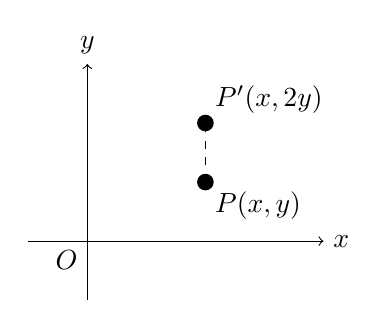
\begin{tikzpicture}[scale=1.5]
    % 绘制坐标轴
    \draw[->] (-0.5,0) -- (2,0) node[right] {$x$};
    \draw[->] (0,-0.5) -- (0,1.5) node[above] {$y$};

    % 绘制原点O
    \coordinate (O) at (0,0);
    \fill (O) circle (0pt) node[anchor=north east] {$O$};
    
    % 绘制旋转前的点P
    \coordinate (P) at (1,0.5);
    \fill (P) circle (2pt) node[anchor=north west] {$P(x, y)$};
    
    % 绘制旋转后的点P'
    \coordinate (P') at (1,1);
    \fill (P') circle (2pt) node[anchor=south west] {$P'(x, 2y)$};
    
    % 绘制连接线和旋转弧
    \draw[dashed] (P) -- (P');
    % \draw[->] (0.5,0.5) -- (0.5,1);
    
\end{tikzpicture}
\caption{伸缩变换示意图\label{fig:伸缩变换}}
\end{figure}

\begin{exercise}

    将直角坐标系 $O x y$ 内每个点的横坐标变为原来的 $k_1$ 倍, 纵坐标变为原来的 $k_2$ 倍 $\left(k_1, k_2\right.$ 均为非零常数) 的伸缩变换, 其坐标变换公式是
    
    \begin{equation}
        \left\{\begin{array}{l}
    x^{\prime}=k_1 x, \\
    y^{\prime}=k_2 y .
    \end{array}\right.
    \label{伸缩变换一般表达式}
    \end{equation}
    
    对应的变换矩阵为 
    
    \begin{equation}
    \left(\begin{array}{cc}k_1 & 0 \\ 0 & k_2\end{array}\right).
    \label{伸缩变换一般矩阵}
    \end{equation}

\end{exercise}

注意到,当$k_1=k_2$时,伸缩变换退化为\textcolor{third}{\bf 平移变换}。


\subsubsection{投影变换}
\label{subsubsec:投影变换}

设 $l$ 是平面内一条给定的直线. 对平面内的任意一点 $P$ 作直线 $l$ 的垂线, 垂足为点 $P^{\prime}$, 则称点 $P^{\prime}$ 为点 $P$ 在直线 $l$ 上的\textcolor{third}{\bf 投影} (projection). 将平面上每一点 $P$ 变成它在直线 $l$ 上的投影 $P^{\prime}$, 这个变换称为关于直线 $l$ 的\textcolor{third}{\bf 投影变换}  .

如图 \ref{fig:投影变换}, 在直角坐标系 $O x y$ 内, 过任意一点 $P$ 作 $x$ 轴的垂线, 垂足为点 $P^{\prime}$, 我们称点 $P^{\prime}$ 为点 $P$ 在 $x$ 轴上的  投影. 如果一个变换把直角坐标系内的每一点变成它在 $x$ 轴上 的投影, 那么称这个变换为关于 $x$ 轴的投影变换.

\begin{figure}[h]
\centering
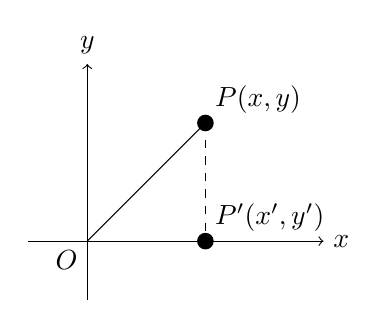
\begin{tikzpicture}[scale=1.5]
    % 绘制坐标轴
    \draw[->] (-0.5,0) -- (2,0) node[right] {$x$};
    \draw[->] (0,-0.5) -- (0,1.5) node[above] {$y$};
    
    % 绘制原点O
    \coordinate (O) at (0,0);
    \fill (O) circle (0pt) node[anchor=north east] {$O$};
    
    % 绘制旋转前的点P
    \coordinate (P) at (1,1);
    \fill (P) circle (2pt) node[anchor=south west] {$P(x, y)$};
    
    % 绘制旋转后的点P'
    \coordinate (P') at (1,0);
    \fill (P') circle (2pt) node[anchor=south west] {$P'(x', y')$};
    
    % 绘制连接线和旋转弧
    \draw[-] (O) -- (P);
    \draw[dashed] (P) -- (P');
    
\end{tikzpicture}
\caption{投影变换示意图\label{fig:投影变换}}
\end{figure}

设在关于 $x$ 轴的投影变换的作用下, 点 $P(x, y)$ 变成 点 $P^{\prime}\left(x^{\prime}, y^{\prime}\right)$。
此时 $x^{\prime}, y^{\prime}$ 与 $x, y$ 有如下关系:

$$
\left\{\begin{array}{l}
x^{\prime}=x, \\
y^{\prime}=0 .
\end{array}\right.
$$

即

$$
\left\{\begin{array}{l}
x^{\prime}= 1 \cdot x + 0 \cdot y, \\
y^{\prime}= 0 \cdot x + 0 \cdot y.
\end{array}\right.
$$

对应的二阶矩阵为 $\left(\begin{array}{ll}1 & 0 \\ 0 & 0\end{array}\right)$.

\subsubsection{切变变换}
\label{subsubsec:切变变换}

\textcolor{third}{\bf 切变变换}(shearing)是一种特殊的几何变换,用于改变物体的形状。它在一个方向上按照一定的比例“拉伸”或“压缩”物体,同时在与这个方向垂直的另一方向上保持物体不变。在二维平面上,切变变换主要有两种:

\begin{itemize}
    \item \textbf{水平切变}:在水平方向上拉伸或压缩物体,与物体在垂直方向上的位置成比例。垂直方向上的形状不会改变。如图\ref{fig:shearing-wiki}\footnote{图源:\url{https://en.wikipedia.org/wiki/Shear\_mapping}}所示。
    \item \textbf{垂直切变}:在垂直方向上拉伸或压缩物体,与物体在水平方向上的位置成比例。水平方向上的形状不会改变。
\end{itemize}


\begin{figure}[!h]
    \centering
    \includegraphics[width=0.4\textwidth]{figure/matrix/shearing.png}
    \caption{平面的水平剪切,将蓝色转变为红色,黑点为原点}
    \label{fig:shearing-wiki}
\end{figure}


如图 \ref{fig:切变变换}, 在直角坐标系 $O x y$ 内, 将每一点 $P(x$, $y$ ) 沿着与 $x$ 轴平行的方向平移 $k y$ 个单位变成点 $P^{\prime}$, 其中 $k$ 是非零常数, 这就是水平切变(或平行于 $x$ 轴的切变变换).
设 $P^{\prime}\left(x^{\prime}, y^{\prime}\right)$, 则
此时 $x^{\prime}, y^{\prime}$ 与 $x, y$ 有如下关系:

$$
\left\{\begin{array}{c}
x^{\prime}=x+k y, \\
y^{\prime}=y .
\end{array}\right.
$$

从而, 对应的二阶矩阵为 $\left(\begin{array}{ll}1 & k \\ 0 & 1\end{array}\right)$.

\begin{figure}[h]
\centering
\begin{tikzpicture}[scale=1.5]
    % 绘制坐标轴
    \draw[->] (-0.5,0) -- (1.5,0) node[right] {$x$};
    \draw[->] (0,-0.5) -- (0,1.5) node[above] {$y$};
    
    % 绘制原点O
    \coordinate (O) at (0,0);
    \fill (O) circle (0pt) node[anchor=north east] {$O$};
    
    % 绘制旋转前的点P
    \coordinate (P) at (0.5,1);
    \fill (P) circle (2pt) node[anchor=south west] {$P(x, y)$};
    
    % 绘制旋转后的点P'
    \coordinate (P') at (1.5,1);
    \fill (P') circle (2pt) node[anchor=south west] {$P'(x+ky, y)$};
    
    % 绘制连接线和旋转弧
    \draw[dashed] (P) -- (P');
    
\end{tikzpicture}
\caption{切变变换示意图\label{fig:切变变换}}
\end{figure}

\begin{exercise}

    平行于 $y$ 轴的切变变换是指将直角坐标系内的每一点 $P(x, y)$ 沿着与 $y$ 轴 平行的方向平移 $k x$ 个单位 (其中 $k$ 是非零常数) 的线性变换. 其坐标变换公式为
    $$
    \left\{\begin{array}{c}
    x^{\prime}=x, \\
    y^{\prime}=k x+y .
    \end{array}\right.
    $$
    对应的矩阵为 $\left(\begin{array}{ll}1 & 0 \\ k & 1\end{array}\right)$.
        
\end{exercise}

\subsection{线性变换与线性空间}

从高中开始我们就熟知平面直角坐标系,这是由两条相互平行、且各自向正、负两个方向无限延伸的横轴、纵轴构成的坐标体系。横轴和纵轴均可以在实数域$\mathbb{R}$上任意取值,故我们可以将平面记作$\mathbb{R}^2 = \mathbb{R}\times\mathbb{R}$。通过第\ref{subsec:几种特殊几何变换}节的例子,我们了解到,二维空间上的点之间可以通过几何变换到达彼此,同时,所得结果也一定还是二维空间中的点。如果我们从原点出发,引一条到特定点的有向箭头,就可以将点表示为向量。因此,之前所列举的几何变换做的事情都是将平面向量变换为其他平面向量。高中时,我们学习过平面向量的加法和数量乘法,我们先来复习一下。

\begin{definition}[平面向量的加法]
  设向量 $\boldsymbol{u}=\left(\begin{array}{l}x_1 \\ y_1\end{array}\right), \boldsymbol{v}=\left(\begin{array}{l}x_2 \\ y_2\end{array}\right)$, 
  向量 $\boldsymbol{u}$ 与 $\boldsymbol{v}$ 的加法满足平行四边形法则,数学表示为 $\boldsymbol{u}+\boldsymbol{v}=\left(\begin{array}{l}x_1+x_2 \\ y_1+y_2\end{array}\right)$.
\end{definition}

\begin{note}
向量加法就是高中学的平行四边形法则。
\end{note}

\begin{definition}[平面向量的数量乘法]
  设向量 $\boldsymbol{u}=\left(\begin{array}{l}x \\ y\end{array}\right)$, 
  规定实数 $\lambda$ 与向量 $\boldsymbol{u}$ 的乘积 $\lambda \boldsymbol{u}=\left(\begin{array}{l}\lambda x \\ \lambda y\end{array}\right)$;
\end{definition}

平面向量的数量乘法之所以被称为"数量乘法"是因为它涉及到一个向量与一个数(或者我们可以称之为标量)相乘的操作。这个数可以是任何实数。当我们将一个向量与一个数相乘时,结果是一个新的向量,它的方向与原始向量相同(或相反),但长度(或称为模)被缩小或拉大了。这个操作影响到向量的大小,所以我们称之为"数量乘法"。


\begin{exercise}

  \begin{enumerate}
    \item   【高中数学人教A版选修4-2】设向量 $\boldsymbol{u}=\left(\begin{array}{l}1 \\ 2\end{array}\right), \boldsymbol{v}=\left(\begin{array}{l}2 \\ 1\end{array}\right)$. 
            如图 \ref{fig:vector-addition-reflection}, 先利用平行四边形法则求 $\boldsymbol{u}+\boldsymbol{v}$, 再对向量 $(\boldsymbol{u}+\boldsymbol{v})$ 进行关于 $x$ 轴的反射变换;
            或者, 先对向量 $\boldsymbol{u}, \boldsymbol{v}$ 做关于 $x$ 轴的反射变换, 
            再利用平行四边形法则求反射变换后的两个向量的和.请回答下列问题:

            \begin{enumerate}
              \item 这两个过程的结果相同吗?
              \item 如果把$\boldsymbol{u}$关于$x$轴的反射变换记作$\text{Reflect}_{x}(\boldsymbol{u})$,
              把$\boldsymbol{v}$关于$x$轴的反射变换记作$\text{Reflect}_{x}(\boldsymbol{v})$,
              把$\boldsymbol{u}+\boldsymbol{v}$关于$x$轴的反射变换记作$\text{Reflect}_{x}(\boldsymbol{u}+\boldsymbol{v})$,
              那么,这些变换的坐标变换矩阵分别是什么?这些变换的矩阵有什么关系?
            \end{enumerate}

            \begin{figure}[!h]
            \centering
            \begin{tikzpicture}[scale=1, transform shape]

              % First diagram: Vector addition first, then reflection
              \begin{scope}[shift={(0,0)}]

                \foreach \x in {-1,0,...,4} {
                  \ifnum \x = 0
                  \else
                        \ifnum \x = 3
                            \draw (\x, 0.1) -- (\x, -0.1) node[below right] {\x};
                        \else
                            \draw (\x, 0.1) -- (\x, -0.1) node[below] {\x};
                        \fi
                  \fi
                }

                \foreach \y in {-3,-2,...,3} {
                    \ifnum \y = 0
                    \else
                        \draw (0.1, \y) -- (-0.1, \y) node[left] {\y};
                    \fi
                }

                % Draw origin
                \node at (0,0) [below left] {$O$};

                % Draw axes
                \draw[thick,->] (-1.5,0) -- (4.5,0) node[anchor=north west] {$x$};
                \draw[thick,->] (0,-3.5) -- (0,3.5) node[anchor=south east] {$y$};
              
                % Draw original vectors alpha and beta
                \draw[thick,->,blue] (0,0) -- (1,2) node[anchor=south] {$\boldsymbol{u}$};
                \draw[thick,->,red] (0,0) -- (2,1) node[anchor=west] {$\boldsymbol{v}$};

                \draw[thick,-,blue,dashed] (1,2) -- (3,3);
                \draw[thick,-,red,dashed] (2,1) -- (3,3);
              
                % Draw alpha + beta
                \draw[thick,->,mygreen] (0,0) -- (3,3) node[anchor=south] {$\boldsymbol{u}+\boldsymbol{v}$};
              
                % Draw reflection of alpha + beta
                \draw[thick,->,mygreen,dashed] (0,0) -- (3,-3) node[anchor=north] {$\text{Reflect}_{x}(\boldsymbol{u}+\boldsymbol{v})$};

                \draw[thick,-,black,dashed] (3,3) -- (3,-3);

                % Add a right-angle symbol (perpendicular mark)
                \draw (3,0) -- (3,0.1) -- (3+0.1,0.1) -- (3+0.1,0);

              \end{scope}
              
              % Second diagram: Reflection first, then vector addition
              \begin{scope}[shift={(7,0)}]

                \foreach \x in {-1,0,...,4} {
                  \ifnum \x = 0
                    % Do nothing when \x is 0
                  \else
                    \ifnum \x = 1
                      \draw (\x, 0.1) -- (\x, -0.1) node[below right] {\x};
                    \else
                      \ifnum \x = 2
                        \draw (\x, 0.1) -- (\x, -0.1) node[below right] {\x};
                      \else
                        \draw (\x, 0.1) -- (\x, -0.1) node[below] {\x};
                      \fi
                    \fi
                  \fi
                }                

                \foreach \y in {-3,-2,...,3} {
                    \ifnum \y = 0
                    \else
                        \ifnum \y = -2
                            \draw (0.1, \y) -- (-0.1, \y) node[above left] {\y};
                        \else
                            \draw (0.1, \y) -- (-0.1, \y) node[left] {\y};
                        \fi
                    \fi
                  }

                % Draw origin
                \node at (0,0) [below left] {$O$};

                % Draw axes
                \draw[thick,->] (-1.5,0) -- (4.5,0) node[anchor=north west] {$x$};
                \draw[thick,->] (0,-3.5) -- (0,3.5) node[anchor=south east] {$y$};

                % Draw original vectors alpha and beta
                \draw[thick,->,blue] (0,0) -- (1,2) node[anchor=south] {$\boldsymbol{u}$};
                \draw[thick,->,red] (0,0) -- (2,1) node[anchor=west] {$\boldsymbol{v}$};
              
                % Draw reflection of alpha and beta
                \draw[thick,->,blue,dashed] (0,0) -- (1,-2) node[anchor=north east] {$\text{Reflect}_{x}(\boldsymbol{u})$};
                \draw[thick,->,red,dashed] (0,0) -- (2,-1) node[anchor=west] {$\text{Reflect}_{x}(\boldsymbol{v})$};

                \draw[thick,-,blue,dashed] (1,-2) -- (3,-3);
                \draw[thick,-,red,dashed] (2,-1) -- (3,-3);

                \draw[thick,-,black,dashed] (1,2) -- (1,-2);
                \draw[thick,-,black,dashed] (2,1) -- (2,-1);
                
                % Add a right-angle symbol (perpendicular mark)
                \draw (1,0) -- (1,0.1) -- (1+0.1,0.1) -- (1+0.1,0);
                \draw (2,0) -- (2,0.1) -- (2+0.1,0.1) -- (2+0.1,0);

                % Draw addition of reflected alpha and beta
                \draw[thick,->,mygreen] (0,0) -- (3,-3) node[anchor=north] {$\text{Reflect}_{x}(\boldsymbol{u}) + \text{Reflect}_{x}(\boldsymbol{v})$};

              \end{scope}

            \end{tikzpicture}
            \caption{向量加法与反射变换}
            \label{fig:vector-addition-reflection}
            \end{figure}

  \item 设向量 $\boldsymbol{u}=\left(\begin{array}{l}2 \\ 1\end{array}\right)$ ,
        如图 \ref{fig:vector-scaling}, 先用$2$与该向量进行数量乘法,再使向量在 \( x \)-轴方向的坐标变为原来的 3 倍,同时使 \( y \)-轴方向的坐标变为原来的 2 倍;
        或者,先使向量在 \( x \)-轴方向的坐标变为原来的 3 倍,同时使 \( y \)-轴方向的坐标变为原来的 2 倍,再用$2$与该向量进行数量乘法。
        请回答下列问题:

        \begin{enumerate}
          \item 这两个过程的结果相同吗?
          \item 如果把$\boldsymbol{u}$的伸缩变换记作$\text{Stretch}(\boldsymbol{u})$,
          把$2\boldsymbol{u}$的伸缩变换记作$\text{Stretch}(2\boldsymbol{u})$,
          那么,这些变换的坐标变换矩阵分别是什么?这些变换的矩阵有什么关系?
        \end{enumerate}

        \begin{figure}[!h]
          \centering
          \begin{tikzpicture}[scale=1, transform shape]

            \foreach \x in {1,2,...,12} {
                \draw (\x, 0.1) -- (\x, -0.1) node[below] {\x};
            }

            \foreach \y in {1,2,...,4} {
                \draw (0.1, \y) -- (-0.1, \y) node[left] {\y};
            }

            % 绘制原点O
            \node at (0,0) [below left] {$O$};

            % Draw axes
            \draw[thick,->] (-0.5,0) -- (12.5,0) node[right] {$x$};
            \draw[thick,->] (0,-0.5) -- (0,4.5) node[above] {$y$};
          
            % Original vector v
            \draw[thick,->,blue] (0,0) -- (2,1) node[above] {$\boldsymbol{u}$};
            
            % Scaled vector 2v
            \draw[thick,->,red] (0,0) -- (4,2) node[above] {$2\boldsymbol{u}$};
          
            % Transformed vector T(v)
            \draw[thick,->,mygreen] (0,0) -- (6,2) node[above] {$\text{Stretch}_{x}(\boldsymbol{u})$};
          
            % Transformed vector T(2v)
            \draw[thick,->,orange] (0,0) -- (12,4) node[above] {$\text{Stretch}_{x}(2\boldsymbol{u})$};
          
          \end{tikzpicture}
          \caption{向量伸缩变换}
          \label{fig:vector-scaling}
        \end{figure}

  \end{enumerate}

\end{exercise}

现在,我们希望将第\ref{subsec:几种特殊几何变换}节中的几何变换抽象为更加一般的形式,这些一般的变换可能没有类似反射变换、旋转变换那样明确的意义,但能够保持几何图形的一些重要性质,如直线的形状、直线之间的平行性、相交直线的交点以及直线上不同点之间的相对距离等。

\begin{note}
  让学生回顾之前展示的每个变换,并提醒他们每个变换都保持了直线的性质。
\end{note}

\begin{proposition}[平面上保持直线性质的变换]
\label{thm:保持直线性质的变换}
设 $T$ 是一个平面到平面的映射($T: \mathbb{R}^2 \rightarrow \mathbb{R}^2$), $\boldsymbol{u}, \boldsymbol{v}$ 是平面上的任意两个向量, $\lambda$ 是一个任意实数。若从原点引出向量$\boldsymbol{u}, \boldsymbol{v}$,其末端点分别记为$P_1,P_2$,显然,只要选取合适的$\boldsymbol{u}, \boldsymbol{v}$,$P_1,P_2$就可以确定出平面上的任意直线。如果 $T$ 满足下面的条件:
\begin{enumerate}
    \item 保加法:$T(\boldsymbol{u}+\boldsymbol{v}) = T(\boldsymbol{u})+T(\boldsymbol{v})$;
    \item 保数乘:$T(\lambda \boldsymbol{u}) =\lambda T(\boldsymbol{u})$.
\end{enumerate}
则该映射不改变直线的形状、平行性、与其他直线的交叉点的位置以及直线上点的相对距离。
\end{proposition}

\begin{proof}

\underline{1. 不改变直线的形状}:直线可以表示为向量的线性组合,即对于两个向量 \(\boldsymbol{u}\) 和 \(\boldsymbol{v}\),直线可以表示为 \(\boldsymbol{u} + t\boldsymbol{v}\),其中 \(t\) 是标量。根据变换$T$的定义,我们有:

\begin{align*}
    T(\boldsymbol{u} + t\boldsymbol{v})
    = & T(\boldsymbol{u}) + T(t\boldsymbol{v})\\
    = & T(\boldsymbol{u}) + tT(\boldsymbol{v})
\end{align*}

即直线在经过这样的变换后仍然是一条直线。

\underline{2. 保持平行性}:考虑两条平行直线,它们可以表示为 \(\boldsymbol{u} + t\boldsymbol{v}\) 和 \(\boldsymbol{u}' + t\boldsymbol{v}\),注意这两条直线共享同一个方向向量 \(\boldsymbol{v}\)。因为变换$T$保持向量加法和标量乘法,变换后的直线分别是 \(T(\boldsymbol{u}) + tT(\boldsymbol{v})\) 和 \(T(\boldsymbol{u}') + tT(\boldsymbol{v})\)。因为它们仍然共享同一个方向向量 \(T(\boldsymbol{v})\),所以变换后的直线保持平行。

\underline{3. 保持交叉点位置}:假设两条直线 \(L_1\) 和 \(L_2\) 在点 \(\boldsymbol{p}\) 交叉,即存在某个 \(t_1\) 和 \(t_2\) 使得 \(\boldsymbol{u} + t_1\boldsymbol{v} = \boldsymbol{u}' + t_2\boldsymbol{v}' = \boldsymbol{p}\)。应用变换 \(T\),我们得到 \(T(\boldsymbol{u} + t_1\boldsymbol{v}) = T(\boldsymbol{u}') + t_2T(\boldsymbol{v}') = T(\boldsymbol{p})\)。这表明变换后的直线在 \(T(\boldsymbol{p})\) 点交叉,保持了交叉点的位置。

\underline{4. 保持直线上点的相对距离}:考虑直线 \(L\) 上的两点 \(\boldsymbol{p}\) 和 \(\boldsymbol{q}\),直线上的任意一点 \(\boldsymbol{x}\) 可以表示为 \(\boldsymbol{p}\) 和 \(\boldsymbol{q}\) 的线性组合:
\[ \boldsymbol{x} = \alpha\boldsymbol{p} + (1-\alpha)\boldsymbol{q} \]
其中,\(\alpha\) 是一个标量。我们将线性变换 \(T\) 应用于直线 \(L\) 上的点 \(\boldsymbol{x}\):
\begin{align*}
    T(\boldsymbol{x}) 
    & = T(\alpha\boldsymbol{p} + (1-\alpha)\boldsymbol{q}) \\
    & = \alpha T(\boldsymbol{p}) + (1-\alpha)T(\boldsymbol{q})    
\end{align*}

这表明,经过线性变换 \(T\) 后,点 \(\boldsymbol{x}\) 依然位于 \(T(\boldsymbol{p})\) 和 \(T(\boldsymbol{q})\) 定义的直线上,并且保持了与原始直线相同的比例 \(\alpha\)。

\end{proof}

到这里,我们证明了平面($\mathbb{R}^2$)上保加法和保数乘的变换的向量映射(或称变换)不会改变直线的形状、直线之间的平行和相交关系,也不会改变直线上的点之间的相对距离,我们称这些性质是平面的“线性”性质,而变换$T$可以在变换前后保持这种“线性”性质,所以,我们称变换$T$为平面上的\textcolor{third}{\bf 线性变换}。

可以验证,在三维空间($\mathbb{R}^3$)中,保加法和保数乘的变换仍然可以保持空间的线性性质,这是三维空间上的线性变换(到了$\mathbb{R}^3$中,线性变换不仅能够直线的的性质不变,还可以保持平面的性质不变)。现在,我们希望将研究对象从我们熟悉的二维、三维空间推广到任意维度。我们注意到,在二维空间中,变换$T$映射的结果向量一定还在二维空间中;在三维空间中,变换$T$映射的结果向量一定还在三维空间中。据此,我们在心中勾勒出一个任意维空间的“印象”,我们希望,\textbf{在这样的空间中,变换$T$映射的结果向量仍然属于同一空间},这样,我们可以得到$\mathbb{R}^4, \mathbb{R}^5$直到$\mathbb{R}^n$。在Gilbert Strang的线性代数教材中就直接使用这种“印象”来定义$\mathbb{R}^n$。

\begin{definition}[$\mathbb{R}^n$]
    $\mathbb{R}^n$是包含所有具有$n$个分量的向量的空间。\\
    The space $\mathbb{R}^n$ consists of all column vectors $v$ with $n$ components.\\
    —— \textbf{Introduction to Linear Algebra} by \textit{Gilbert Strang}
\end{definition}

可以证明,\ref{thm:保持直线性质的变换}中的变换$T$在$\mathbb{R}^n$仍然能够保持空间的线性性质,所以变换$T$也是$\mathbb{R}^n$中的线性变换。在$\mathbb{R}^n$中,如果要保证线性变换的结果向量仍然在$\mathbb{R}^n$中,需要满足如下的条件:
\begin{itemize}
    \item 对向量加法满足:
    \begin{itemize}
        \item 加法交换律$\boldsymbol{\alpha}+\boldsymbol{\beta} = \boldsymbol{\beta}+\boldsymbol{\alpha}$;
        \item 加法结合律$(\boldsymbol{\alpha}+\boldsymbol{\beta})+\boldsymbol{\gamma}=\boldsymbol{\alpha}+(\boldsymbol{\beta}+\boldsymbol{\gamma})$;
        \item 存在零元,因为要保证$\exists \boldsymbol{x}\text{, s.t. } \boldsymbol{\alpha}+\boldsymbol{x}=\boldsymbol{\alpha}$,这时候$\boldsymbol{x}$就是零元,记为$\boldsymbol{0}$;
        \item 存在逆元,因为要保证$\exists \boldsymbol{x}\text{, s.t. } \boldsymbol{\alpha}+\boldsymbol{x}=\boldsymbol{0}$,这时候$\boldsymbol{x}$就是$\boldsymbol{\alpha}$的逆元,记为$-\boldsymbol{\alpha}$;
    \end{itemize}
    \item 对向量数乘满足:
    \begin{itemize}
        \item 标量间乘法和数乘的结合性:$k(l\boldsymbol{\alpha}) = (kl)\boldsymbol{\alpha}$;
        \item 存在数乘单位元:$1 \boldsymbol{\alpha} = \boldsymbol{\alpha}$;
    \end{itemize}
    \item 对向量加法和数乘满足:
    \begin{itemize}
        \item 数乘对向量加法的分配律:$k(\boldsymbol{\alpha} + \boldsymbol{\beta}) = k\boldsymbol{\alpha} + k\boldsymbol{\beta}$;
        \item 数乘对标量间加法的分配律:$(k+l)\boldsymbol{\alpha} = k\boldsymbol{\alpha} + l\boldsymbol{\alpha}$;
    \end{itemize}
\end{itemize}

% Here's a specific example where the distributive axiom $a(\boldsymbol{u} + \boldsymbol{v}) = a\boldsymbol{u} + a\boldsymbol{v}$ is not included in the definition of a linear space, resulting in inconsistencies and distortions:

% Consider a set $V = \{\boldsymbol{u}, \boldsymbol{v}\}$ where $\boldsymbol{u} = (1, 0)$ and $\boldsymbol{v} = (0, 1)$, along with a scalar field $\mathbb{R}$. We define vector addition and scalar multiplication as follows:

% Vector addition:
% $\boldsymbol{u} + \boldsymbol{u} = \boldsymbol{u}$
% $\boldsymbol{v} + \boldsymbol{v} = \boldsymbol{v}$
% $\boldsymbol{u} + \boldsymbol{v} = \boldsymbol{v} + \boldsymbol{u} = \boldsymbol{u}$

% Scalar multiplication (violating the distributive axiom):
% $a\boldsymbol{u} = (a, 0)$ for all $a \in \mathbb{R}$
% $a\boldsymbol{v} = (0, a^2)$ for all $a \in \mathbb{R}$

% In this example, the distributive axiom does not hold:

% $a(\boldsymbol{u} + \boldsymbol{v}) = a\boldsymbol{u} = (a, 0)$

% However,
% $a\boldsymbol{u} + a\boldsymbol{v} = (a, 0) + (0, a^2) = (a, a^2)$

% Clearly, $a(\boldsymbol{u} + \boldsymbol{v}) \neq a\boldsymbol{u} + a\boldsymbol{v}$.

% This violation of the distributive axiom leads to inconsistencies and distortions in the geometric properties of the space. For example, if we consider a linear transformation $T$ defined by $T(\boldsymbol{u}) = \boldsymbol{v}$ and $T(\boldsymbol{v}) = \boldsymbol{u}$, then:

% $T(2\boldsymbol{u}) = T((2, 0)) = (0, 4)$

% However,
% $2T(\boldsymbol{u}) = 2\boldsymbol{v} = (0, 4)$

% In this case, the linear transformation $T$ does not preserve the scalar multiplication property, leading to inconsistencies in the geometric properties of the space.

% This example demonstrates that without the distributive axiom, the resulting space does not behave consistently as a linear space, and geometric properties can be distorted or contradictory.

% \begin{proof}
%     要证明线性变换保持形状、平行性和交叉点的位置,我们可以具体考虑两条直线及其在线性变换下的表现。

% \underline{1. 形状保持}:假设有一条直线 \(L_1\),其方程为 \(y = mx + n\),其中 \(m\) 是斜率,\(n\) 是截距。我们考虑两个点 \(P_1(x_1, y_1),P_2(x_2, y_2)\) 在这条直线上,即 \(y_1 = mx_1 + n, y_2 = mx_2 + n\)。

% 现在,应用变换 \(T\),用矩阵表示为 \(\begin{pmatrix} a & b \\ c & d \end{pmatrix}\),于是有
% \[ T(P_1) = \begin{pmatrix} a & b \\ c & d \end{pmatrix} \begin{pmatrix} x_1 \\ mx_1 + n \end{pmatrix},\quad
% T(P_2) = \begin{pmatrix} a & b \\ c & d \end{pmatrix} \begin{pmatrix} x_2 \\ mx_2 + n \end{pmatrix}
% % = \begin{pmatrix} ax + b(mx + n) \\ cx + d(mx + n) \end{pmatrix} 
% % = \begin{pmatrix} (a + bm) x + bn \\ (c + dm)x + dn \end{pmatrix} 
% \]
% 可以验证,变换后的点 \(T(P_1), T(P_2)\) 处在一条斜率为$\frac{bm}{a}$的直线上,这表明原来直线的“形状”(即“直的线”)得到了保持\textcolor{red}{(验证过程留做习题)}。

% \underline{2. 平行性保持}:考虑两条平行直线 \(L_1: y = m_1x + n_1\) 和 \(L_2: y = m_2x + n_2\),因为它们平行,所以 \(m_1 = m_2\)。

% 应用变换 \(T\) 到这两条直线上,我们可以得到新的两条直线。计算出两条新直线的斜率可以发现二者仍然相等,即保持了平行性\textcolor{red}{(验证过程留做习题)}。

% \underline{3. 交叉点保持}:假设两条直线 \(L_1: y = m_1x + n_1\) 和 \(L_2: y = m_2x + n_2\) 交于点 \(P(x, y)\),即满足
% \[ m_1x + n_1 = m_2x + n_2 \]
% 解这个方程可以得到交点 \(P\) 的坐标。在变换 \(T\) 下,两条直线变为 \(T(L_1)\) 和 \(T(L_2)\)。
% 可以验证,\(T(L_1)\) 和 \(T(L_2)\)的交点为$T(P)$\textcolor{red}{(验证过程留做习题)}。
% % 由于线性变换是结构保持的,原有的交点 \(P\) 在变换后的直线上的对应点 \(T(P)\) 保持为这两条新直线的交点。换句话说,如果两条直线在变换前相交,它们在变换后仍然相交于对应的点,这是因为线性变换保持了方程组的解的结构,即交点。

% \end{proof}

% 证明的关键点:

% \begin{itemize}
%     \item 形状保持的证明关键在于展示变换\(T\)的作用下,直线方程仍保持为直线方程,即证明变换后的输出仍满足直线方程的一般形式。
%     \item 平行性保持的证明依赖于展示如果两直线在变换前平行(斜率相等),则在变换后仍然平行。这可以通过比较变换后两条直线的斜率来证明。
%     \item 交叉点保持的证明需要表明如果两直线在变换前有交点,那么在变换后它们仍然会在某点交汇,且该点是原交点变换后的点。
% \end{itemize}

\begin{definition}[线性空间]
\label{def:线性空间}
设 $V$ 是一个非空集合, $\mathcal{F}$ 是一个\textcolor{third}{\bf 数域},在数域$\mathcal{F}$中,\underline{数的加法和乘法}能够顺利按照我们小学所学习的规则进行. 在集合 $V$ 的元素之间定义了一种代数运算,叫做\underline{加法};即给出了一个法则,对于 $V$ 中任意两个元素 $\alpha$ 与 $\boldsymbol{\beta}$, 在 $V$ 中都有唯一的一个元素 $\gamma$与它们对应,称为 $\boldsymbol{\alpha}$ 与 $\boldsymbol{\beta}$ 的和, 记为 $\gamma=\alpha+\boldsymbol{\beta}$. 在数域 $\mathcal{F}$ 与集合 $V$的元素之间还定义了一种运算, 叫做\underline{数量乘法};这就是说, 对于数域 $\mathcal{F}$ 中任一数 $k$ 与 $V$ 中任一元素 $\alpha$, 在 $V$ 中都有唯一的一个元素$\delta$与它们对应, 称为 $k$ 与 $\alpha$ 的数量乘积, 记为 $\delta=k \boldsymbol{\alpha}$. 如果加法与数量乘法满足上面8条规则, 那么 $V$ 称为数域 $\mathcal{F}$ 上的\textcolor{third}{\bf 线性空间}(也称\textcolor{third}{\bf 向量空间}).
\end{definition}

定义中,数域这一概念的严格定义一般在抽象代数课程里讨论,我们这里将其理解为一个保证加法和乘法能够顺利进行的数的集合即可。可以将其想象为一种“通用货币系统”,在这个系统里,我们可以自由地进行交易(加法和乘法运算)而不用担心交换规则突然改变。就像在日常生活中,无论我们是在商店购物还是在银行存取款项,货币的基本价值和使用规则保持不变,使得经济交易可以顺利进行。

\vspace{0.3cm}

\begin{note}
    线性空间的定义可以简记为:对加法和数量乘法满足封闭性+8条公理。实际上这个定义是有冗余的,因为满足封闭性就必须要有8条公理。
\end{note}

\vspace{0.3cm}

为什么要煞有介事的重新定义加法和数量乘法,显得多此一举,直接用平面向量的加法和数量乘法不行吗?确实不行,因为定义\ref{def:线性空间}中集合$V$的元素不一定是数字或我们上面讨论的各种空间中的向量,即我们希望传达一个观点,一大类数学对象各自形成的集合都是线性空间。下面举几个例子:

\textbf{1. 多项式空间。}多项式空间是所有具有特定最高次数的多项式的集合。例如,考虑所有最高次数为 2 的实系数多项式的集合,记为 \(P_2(\mathbb{R})\)。这个空间包括形如 \(ax^2 + bx + c\) 的所有多项式,其中 \(a, b, c\) 是实数系数。

\begin{itemize}
    \item 向量加法:两个多项式相加,就是它们对应系数的和。例如,如果我们有 \(p_1(x) = 2x^2 + 3x + 1\) 和 \(p_2(x) = x^2 - 2x + 4\),它们的和 \(p_1(x) + p_2(x) = (2x^2 + x^2) + (3x - 2x) + (1 + 4) = 3x^2 + x + 5\) 也在 \(P_2(\mathbb{R})\) 中。
    \item 标量乘法:一个多项式乘以一个标量,就是每个系数乘以这个标量。例如,如果 \(k = 3\) 和 \(p_1(x) = 2x^2 + 3x + 1\),则 \(kp_1(x) = 3(2x^2 + 3x + 1) = 6x^2 + 9x + 3\)。
\end{itemize}

\textbf{2. 实函数空间。}考虑所有定义在实数上,取值也为实数的连续函数的集合,记为 \(C(\mathbb{R})\)。这是一个非常广泛的向量空间,包括如直线、抛物线等基本函数。

\begin{itemize}
    \item 向量加法:两个函数的和是一个新的函数,其值在每一点上都是原来两个函数值的和。例如,如果 \(f(x) = x^2\) 和 \(g(x) = 2x\),那么它们的和 \(h(x) = f(x) + g(x) = x^2 + 2x\)。
    \item 标量乘法:一个函数乘以一个标量,结果是一个新的函数,其值在每一点上都是原来函数值乘以该标量。例如,如果 \(k = 2\) 和 \(f(x) = x^2\),那么 \(kf(x) = 2f(x) = 2x^2\)。
\end{itemize}

\textbf{3. 实矩阵空间。}考虑所有 \(2 \times 2\) 的实数矩阵的集合,记为 \(M_{2,2}(\mathbb{R})\)。这个空间包括所有形如 \(\begin{pmatrix} a & b \\ c & d \end{pmatrix}\) 的矩阵,其中 \(a, b, c, d\) 是实数。

\begin{itemize}
    \item 向量加法:两个矩阵相加,就是它们对应元素的和。例如,如果我们有 \(A = \begin{pmatrix} 1 & 2 \\ 3 & 4 \end{pmatrix}\) 和 \(B = \begin{pmatrix} 4 & 3 \\ 2 & 1 \end{pmatrix}\),它们的和 \(A + B = \begin{pmatrix} 1+4 & 2+3 \\ 3+2 & 4+1 \end{pmatrix} = \begin{pmatrix} 5 & 5 \\ 5 & 5 \end{pmatrix}\)。
    \item 标量乘法:一个矩阵乘以一个标量,就是每个元素乘以这个标量。例如,如果 \(k = 2\) 和 \(A = \begin{pmatrix} 1 & 2 \\ 3 & 4 \end{pmatrix}\),则 \(kA = 2 \cdot \begin{pmatrix} 1 & 2 \\ 3 & 4 \end{pmatrix} = \begin{pmatrix} 2 & 4 \\ 6 & 8 \end{pmatrix}\)。
\end{itemize}

\begin{definition}[线性变换]
    \textcolor{third}{\bf 线性变换}是从一个线性空间到另一个线性空间的映射 \(\mathcal{A}: V \rightarrow W\),对于所有的 \(\boldsymbol{\alpha}, \boldsymbol{\beta} \in V\) 和任意标量 \(k_1, k_2\),满足以下两个条件:

    \begin{enumerate}
        \item \textbf{加法保持性:}\(\mathcal{A}(\boldsymbol{\alpha} + \boldsymbol{\beta}) = \mathcal{A}(\boldsymbol{\alpha}) + \mathcal{A}(\boldsymbol{\beta})\)
        \item \textbf{数量乘法保持性:}\(\mathcal{A}(k\boldsymbol{\alpha}) = k\mathcal{A}(\boldsymbol{\alpha})\)
    \end{enumerate}
\end{definition}

上述两条可以写成一条:设 $\mathcal{A}$ 是平面上一个线性变换, $\boldsymbol{\alpha}, \boldsymbol{\beta}$ 是平面上的任意两个向量, $k_1, k_2$ 是任意两个 实数, 则
\begin{equation}
  \mathcal{A}\left(k_1 \boldsymbol{\alpha}+k_2 \boldsymbol{\beta}\right)=k_1 \mathcal{A} (\boldsymbol{\alpha})+k_2 \mathcal{A} (\boldsymbol{\beta})
\end{equation}

\section{矩阵的运算}

\begin{note}
矩阵乘法的规则是\textcolor{red}{“行乘列”}。这一点在计算结果时很重要,但无助于理解矩阵乘法的本质,我们应该从线性变换和线性组合的角度理解矩阵乘法。
\end{note}

\subsection{向量与向量间的乘法运算}

在介绍矩阵的运算之前我们首先回顾向量之间的乘法运算。存在两种类型的向量与向量的乘积:内积和外积。

\begin{definition}[内积] \label{def:inner-product} 
对 $x, y \in \mathbb{R}^n$, 我们有:
$$
x^T y=\sum_{i=1}^n x_i y_i \in \mathbb{R}
$$
\end{definition}

\begin{exercise}\label{exer:01}
假设我们有两个二维向量 $x = \begin{bmatrix} 1 \\ 2 \end{bmatrix}$ 和 $y = \begin{bmatrix} 3 \\ 4 \end{bmatrix}$。我们可以使用定义 \ref{def:inner-product} 中的公式来计算它们的内积:

\[
x^T y = x y^T = \begin{bmatrix} 1 & 2 \end{bmatrix} \begin{bmatrix} 3 \\ 4 \end{bmatrix} = (1 \cdot 3) + (2 \cdot 4) = 3 + 8 = 11
\]

因此,向量 $x$ 和 $y$ 的内积为 $11$。
\end{exercise}

\begin{definition}[外积] \label{def:outer-product} 
对 $x \in \mathbb{R}^m, y \in \mathbb{R}^n$, 我们有:
$$
x y^T=\left(\begin{array}{ccc}
x_1 y_1 & \cdots & x_1 y_n \\
\vdots & & \vdots \\
x_m y_1 & \cdots & x_m y_n
\end{array}\right) \in \mathbb{R}^{m \times n}
$$
\end{definition}

\begin{exercise}
    假设我们有一个列向量 $x = \begin{bmatrix} 1 \\ 2 \end{bmatrix}$ 和一个三维向量 $y = \begin{bmatrix} 3 \\ 4 \\ 5 \end{bmatrix}$。我们可以使用定义 \ref{def:outer-product} 中的公式来计算它们的外积:

\[
x y^T = \begin{bmatrix} 1 \\ 2 \end{bmatrix} \begin{bmatrix} 3 & 4 & 5 \end{bmatrix}
\]

计算这个外积:

\[
x y^T = \begin{bmatrix}
1 \cdot 3 & 1 \cdot 4 & 1 \cdot 5 \\
2 \cdot 3 & 2 \cdot 4 & 2 \cdot 5 \\
\end{bmatrix} = \begin{bmatrix}
3 & 4 & 5 \\
6 & 8 & 10 \\
\end{bmatrix}
\]

因此,列向量 $x$ 和三维向量 $y$ 的外积是一个 $2 \times 3$ 的矩阵。
\end{exercise}


\subsection{矩阵与向量间的乘法运算}

\begin{note}
    矩阵乘向量就是对向量做某一个线性变换。
\end{note}

\vspace{0.3cm}

在第\ref{subsec:几种特殊几何变换}节中,我们通过将线性变换写成坐标变换方程的方法,
指出平面上线性变换和二阶方阵之间存在着一一对应的关系,即我们实现了用矩阵表示线性变换。

此外,我们之前提到,矩阵源于人们在解方程组是对简洁表达的需求。
那么,不借助坐标变换方程,我们可否直接用矩阵来实现坐标变换呢?答案是肯定的.

让我们回顾一下式(\ref{eq:旋转变换的坐标变换公式}),在直角坐标系 $O x y$ 内, 
将任意一点$P(x, y)$绕原点 $O$ 按逆时针方向旋转 $\theta$ 角得到点$P^{\prime}(x^{\prime}, y^{\prime})$的旋转变换的坐标变换公式

\begin{equation*}
  \left\{\begin{array}{l}
  x^{\prime}=x \cos \theta-y \sin \theta, \\
  y^{\prime}=x \sin \theta+y \cos \theta .
  \end{array}\right.    
\end{equation*}

我们进行如下规定,就可以实现用矩阵来做坐标变换

% Define custom colors
\definecolor{softgreen}{rgb}{0.7, 1.0, 0.7}
\definecolor{softblue}{rgb}{0.7, 0.7, 1.0}
\definecolor{coralred}{rgb}{1.0, 0.5, 0.5}
\definecolor{softorange}{rgb}{1.0, 0.8, 0.6}
\definecolor{softyellow}{rgb}{1.0, 1.0, 0.7}

% % Define custom column types with background colors
% \newcolumntype{S}{>{\columncolor{softgreen}}c}
% \newcolumntype{R}{>{\columncolor{coralred}}c}

\begin{equation}
  \left(\begin{array}{c}
    \cellcolor{softyellow} x^{\prime} \\
    \cellcolor{softorange} y^{\prime}
  \end{array}\right)=\left(\begin{array}{cc}
    \cellcolor{softyellow} \cos \theta & \cellcolor{softyellow} -\sin \theta \\
    \cellcolor{softorange} \sin \theta & \cellcolor{softorange} \cos \theta
    \end{array}\right) \cdot \left(\begin{array}{>{\columncolor{coralred}}c}
  x \\
  y
  \end{array}\right)=\left(\begin{array}{c}
    \cellcolor{softyellow} (\cos \theta) \cdot x + (-\sin \theta) \cdot y \\
    \cellcolor{softorange} (\sin \theta) \cdot x + (\cos \theta) \cdot y
    \end{array}\right)
\label{eq:旋转作为矩阵和向量的乘法的例子}
\end{equation}

我们把第二个等号对应的关系称为\textcolor{third}{\bf 矩阵与向量间的乘法运算}。
将一个矩阵与一个向量相乘,就是对该向量进行该矩阵所表示的线性变换。
\vspace{0.3cm}
\begin{note}
  学生可以尝试把之前的几何变换的坐标变换公式写成矩阵与向量间的乘法运算。
\end{note}

\vspace{0.3cm}

\begin{definition}[矩阵与向量间的乘法运算] \label{def:mat-vec-multi}

矩阵 $A \in \mathbb{R}^{m \times n}$ 和向量 $x \in \mathbb{R}^n$ 的乘积是一个大小为 $\mathbb{R}^m$ 的向量, 满足:

$$
A x=\left(\begin{array}{c}
a_{r, 1}^T x \\
\vdots \\
a_{r, m}^T x
\end{array}\right)=\sum_{i=1}^n a_{c, i} x_i \in \mathbb{R}^m
$$

其中 $a_{r, i}^T$ 是行向量, $a_{c, j}$ 是 $A$ 的列向量, $x_i$ 是 $x$ 的元素。
\end{definition}

\begin{exercise}
    假设我们有一个$2\times 3$的矩阵 $A$ 与一个3维向量 $x$ 相乘。

矩阵 $A$ 和向量 $x$ 的值如下:

\begin{equation*}
A = \begin{bmatrix}
1 & 2 & 3 \\
4 & 5 & 6 \\
\end{bmatrix},\quad
x = \begin{bmatrix}
2 \\
3 \\
1 \\
\end{bmatrix}
\end{equation*}

现在,让我们根据定义,计算 $Ax$ 的乘积:

\begin{equation*}
Ax = \begin{bmatrix}
1 & 2 & 3 \\
4 & 5 & 6 \\
\end{bmatrix} \begin{bmatrix}
2 \\
3 \\
1 \\
\end{bmatrix}
\end{equation*}

我们首先计算每一行与向量 $x$ 的内积,然后将结果组合成一个新的向量:

1. 第一行与 $x$ 的内积: $a_{1,1}^T x = \begin{bmatrix} 1 & 2 & 3 \end{bmatrix} \begin{bmatrix} 2 \\ 3 \\ 1 \end{bmatrix} = 1 \cdot 2 + 2 \cdot 3 + 3 \cdot 1 = 2 + 6 + 3 = 11$

2. 第二行与 $x$ 的内积: $a_{2,1}^T x = \begin{bmatrix} 4 & 5 & 6 \end{bmatrix} \begin{bmatrix} 2 \\ 3 \\ 1 \end{bmatrix} = 4 \cdot 2 + 5 \cdot 3 + 6 \cdot 1 = 8 + 15 + 6 = 29$

因此,$Ax$ 的结果是一个大小为 $\mathbb{R}^2$ 的向量,其元素分别是 $11$ 和 $29$。
\end{exercise}

\begin{exercise}
    假设我们有一个$2\times 2$的矩阵 $A$ 与一个2维向量 $x$ 相乘。

矩阵 $A$ 和向量 $x$ 的值如下:

\begin{equation*}
A = \begin{bmatrix}
1 & 0 \\
0 & 1 \\
\end{bmatrix},\quad
x = \begin{bmatrix}
2 \\
3 \\
\end{bmatrix}
\end{equation*}
\end{exercise}

单位矩阵乘以任何向量等于向量本身,单位矩阵表示恒等变换。

我们注意到,式(\ref{eq:旋转作为矩阵和向量的乘法的例子})还有另一种写法:
\begin{equation}
    \left(\begin{array}{cc}
    \cellcolor{softyellow} \cos \theta & \cellcolor{softorange} -\sin \theta \\
    \cellcolor{softyellow} \sin \theta & \cellcolor{softorange} \cos \theta
    \end{array}\right) \cdot 
    \left(\begin{array}{cc}
      \cellcolor{softyellow}{x} \\
      \cellcolor{softorange}{y}
  \end{array}\right)
    = \hlsoftyellow{$x$} \left(\begin{array}{c}\cellcolor{softyellow}{\cos \theta} \\ \cellcolor{softyellow}{\sin \theta}\end{array}\right) + \hlsoftorange{$y$} \left(\begin{array}{c}\cellcolor{softorange}{-\sin \theta} \\ \cellcolor{softorange}{\cos \theta}\end{array}\right)
\label{eq:旋转作为将矩阵视为列向量线性组合的例子}
\end{equation}

我们称式(\ref{eq:旋转作为将矩阵视为列向量线性组合的例子})为对向量$\left(\begin{array}{c}
\cos \theta \\
\sin \theta
\end{array}\right)$和向量$\left(\begin{array}{c}
-\sin \theta \\
\cos \theta
\end{array}\right)$的\textcolor{third}{\bf 线性组合},$x,y$称为组合系数。
在这个例子中,初学者可能会可能会混淆混淆线性变换和线性组合,线性变换指的是利用
$\left(\begin{array}{cc}
\cos \theta & -\sin \theta \\
\sin \theta & \cos \theta
\end{array}\right)$对
$\left(\begin{array}{c}
x \\
y
\end{array}\right)$进行变换,而线性组合指的是$x,y$作为组合系数对向量$\left(\begin{array}{c}
\cos \theta \\
\sin \theta
\end{array}\right)$和向量$\left(\begin{array}{c}
-\sin \theta \\
\cos \theta
\end{array}\right)$进行组合。
线性组合是理解矩阵和向量的乘法的关键,这是Gilbert Strang的线性代数教材中介绍的第一个概念。下面给出Strang教材中的定义。
\begin{definition}[线性组合]
    The heart of linear algebra is in two operations--both with vectors. We add vectors to get $\boldsymbol{v}+\boldsymbol{w}$. We multiply them by numbers $c$ and $d$ to get $c \boldsymbol{v}$ and $d \boldsymbol{w}$. Combining those two operations (adding $c \boldsymbol{v}$ to $d \boldsymbol{w}$ ) gives the \textcolor{third}{\bf linear combination} $c \boldsymbol{v}+d \boldsymbol{w}$.
\end{definition}

\vspace{0.3cm}

\begin{note}
    特别地,零向量是任何一组向量的线性组合,请思考原因。
\end{note}

\vspace{0.3cm}

有了我们上面的诸多铺垫,我们早已认识到加法和乘法在线性代数中的核心地位,也比较容易理解为什么“线性组合”这一名称中带有“线性”二字,因为这两个操作是线性变换的基本组成部分。线性变换保留向量空间的线性结构,意味着向量加法和标量乘法的结果仍然在原向量空间内。

在上面的例子告诉我们,矩阵和向量的乘法可以视为用向量的每一个分量对矩阵的各个列对应的向量进行线性组合,我们称矩阵的列对应的向量是\textcolor{third}{\bf 矩阵的列向量},当然,对偶地,我们也称矩阵的行对应的向量为\textcolor{third}{\bf 矩阵的行向量}。

\subsection{矩阵与矩阵间的乘法运算}

\begin{note}
    矩阵和矩阵的乘法是两个线性变换的复合。
\end{note}

\vspace{0.3cm}

我们从线性变换的角度引入矩阵和矩阵之间的乘法。我们考虑平面上的点$P(1,0)$,我们首先将其逆时针旋转$90^{\circ}$,对应的变换矩阵为
$
\begin{bmatrix}
0 & -1 \\
1 & 0 \\
\end{bmatrix}
$,
得到点$P^{\prime} (0, 1)$,然后按照$x$轴对称,变换矩阵为
$
\begin{bmatrix}
1 & 0 \\
0 & -1 \\
\end{bmatrix}
$,
得到点$P^{\prime\prime}(0,-1)$。
注意到,这两个变换的复合结果等效于将点$P(1,0)$沿着直线$y=-x$进行反射,该变换的变换矩阵是
$\begin{bmatrix}
0 & -1 \\
-1 & 0 \\
\end{bmatrix}$。
这样的现象在线性空间中普遍存在。因为我们把线性变换的复合在矩阵上的表现抽象出来定义为一种运算,这种运算就是矩阵和矩阵之间的乘法。

\begin{equation*}
    \left(\begin{array}{cc}
    \cellcolor{softyellow}{0} & \cellcolor{softyellow}{-1} \\
    \cellcolor{softorange}{1} & \cellcolor{softorange}{0} \\
    \end{array}\right)
    \cdot
    \left(\begin{array}{cc}
    \cellcolor{softyellow}{1} & \cellcolor{softorange}{0} \\
    \cellcolor{softyellow}{0} & \cellcolor{softorange}{-1} \\
    \end{array}\right)
    =
    \left(\begin{array}{cc}
    \cellcolor{softyellow}{0} & -1 \\
    -1 & \cellcolor{softorange}{0} \\
    \end{array}\right)
\end{equation*}

\begin{definition}[矩阵和矩阵的乘法] \label{def:mat-mat-multi}
    
矩阵 $A \in \mathbb{R}^{m \times n}$ 和 $B \in \mathbb{R}^{n \times p}$ 的乘积是一个大小为 $\mathbb{R}^{n \times p}$ 的矩阵, 满足:

$$
A B=\left(\begin{array}{ccc}
a_{r, 1}^T b_{c, 1} & \cdots & a_{r, 1}^T b_{c, p} \\
\vdots & & \vdots \\
a_{r, m}^T b_{c, 1} & \cdots & a_{r, m}^T b_{c, p}
\end{array}\right)=\sum_{i=1}^n a_{c, i} b_{r, i}^T \in \mathbb{R}^{n \times p}
$$

其中 $a_{r, i}^T, b_{r, i}^T$ 是行向量, $a_{c, j}, b_{c, j}$ 分别是 $A$ 和 $B$ 的列向量。
\end{definition}

\begin{exercise}
    我们将使用一个$2\times 3$的矩阵 $A$ 与一个$3\times 2$的矩阵 $B$ 相乘。

首先,让我们定义矩阵 $A$ 和矩阵 $B$:

\begin{equation*}
A = \begin{bmatrix}
1 & 2 & 3 \\
4 & 5 & 6 \\
\end{bmatrix}
,\quad
B = \begin{bmatrix}
2 & 3 \\
4 & 5 \\
6 & 7 \\
\end{bmatrix}
\end{equation*}

现在,让我们使用这个新的矩阵 $B$ 与之前定义的矩阵 $A$ 相乘,以演示矩阵乘法的过程:

\begin{equation*}
AB = \begin{bmatrix}
1 & 2 & 3 \\
4 & 5 & 6 \\
\end{bmatrix} \begin{bmatrix}
2 & 3 \\
4 & 5 \\
6 & 7 \\
\end{bmatrix}
\end{equation*}

计算每一行与每一列的内积,并生成新的矩阵 $AB$:

1. 第一行与第一列的内积: $a_{1,1}^T b_{1,1} = \begin{bmatrix} 1 & 2 & 3 \end{bmatrix} \begin{bmatrix} 2 \\ 4 \\ 6 \end{bmatrix} = 1 \cdot 2 + 2 \cdot 4 + 3 \cdot 6 = 2 + 8 + 18 = 28$

2. 第一行与第二列的内积: $a_{1,1}^T b_{2,1} = \begin{bmatrix} 1 & 2 & 3 \end{bmatrix} \begin{bmatrix} 3 \\ 5 \\ 7 \end{bmatrix} = 1 \cdot 3 + 2 \cdot 5 + 3 \cdot 7 = 3 + 10 + 21 = 34$

3. 第二行与第一列的内积: $a_{2,1}^T b_{1,1} = \begin{bmatrix} 4 & 5 & 6 \end{bmatrix} \begin{bmatrix} 2 \\ 4 \\ 6 \end{bmatrix} = 4 \cdot 2 + 5 \cdot 4 + 6 \cdot 6 = 8 + 20 + 36 = 64$

4. 第二行与第二列的内积: $a_{2,1}^T b_{2,1} = \begin{bmatrix} 4 & 5 & 6 \end{bmatrix} \begin{bmatrix} 3 \\ 5 \\ 7 \end{bmatrix} = 4 \cdot 3 + 5 \cdot 5 + 6 \cdot 7 = 12 + 25 + 42 = 79$

因此,$AB$ 的结果是一个大小为 $\mathbb{R}^{2 \times 2}$ 的矩阵,其元素如下:

\begin{equation*}
AB = \begin{bmatrix}
28 & 34 \\
64 & 79 \\
\end{bmatrix}
\end{equation*}

\end{exercise}

\subsection{初等变换与矩阵的乘法}
\label{subsec:初等变换与矩阵的乘法}

在第\ref{subsec:高斯-若尔当消元法}节中,我们给出了行变换的概念。事实上,在解方程组的过程中,只有三种基本的行变换:
\begin{itemize}
    \item 行交换(Row-switching transformations): 交换矩阵中的两行;
    \item 行乘以非零系数(Row-multiplying transformations): 将某一行所有的元素乘以一个非零常数;
    \item 行加减(Row-addition transformations): 将某一行的若干倍加到另一行上。
\end{itemize}

我们在单位矩阵上进行三种行变换,看看会发生什么。二阶单位矩阵是一个简单的矩阵,其形式为:

\[ I = \begin{pmatrix} 1 & 0 \\ 0 & 1 \end{pmatrix} \]

这个单位矩阵将作为我们变换的基础。
% 通过对这个单位矩阵应用三种基本的行变换,我们可以生成三种不同的初等矩阵。

\textbf{行交换。}如果我们交换这个单位矩阵的两行,我们得到一个矩阵:

\[ T_{1,2} = \begin{pmatrix} 0 & 1 \\ 1 & 0 \end{pmatrix} \]

$T_{i,j}$表示交换矩阵的第$i$行和第$j$行。

\textbf{行倍乘。}如果我们将第一行乘以一个非零常数,比如2,我们得到:

\[ D_{1}(2) = \begin{pmatrix} 2 & 0 \\ 0 & 1 \end{pmatrix} \]

$D_{i}(m)$代表对矩阵的第$i$行的所有元素乘以标量$m$。按照我们之前的讨论知,它起到伸缩变换的效果。其形式可概括为:除了第 i 个位置(此处为 m)外,所有对角元素均为 1的对角矩阵。

\textbf{行加减。}如果我们将第二行的2倍加到第一行上,我们得到:

\[ L_{12}(2) = \begin{pmatrix} 1 & 2 \\ 0 & 1 \end{pmatrix} \]

矩阵 $L_{ij}(m)$ 将行 $j$ 乘以标量 $m$ 加到行 $i$,其形式可概括为单位矩阵在 $(i, j)$ 位置有一个 $m$。

$T_{i,j}, D_{i}(m)\text{和}L_{ij}(m)$三种矩阵是初等行变换对应的矩阵,我们将其称为\textcolor{third}{\bf 初等矩阵}。
现在,让我们通过一个例子来展示如何使用这些初等矩阵。

\begin{exercise}
考虑一个二阶矩阵\(A\):

\[ A = \begin{pmatrix} 3 & 4 \\ 5 & 6 \end{pmatrix} \]

当我们使用 $T_{1,2} $左边乘矩阵\(A\)(又称\textbf{左乘}\(A\))时,我们有

\[ T_{1,2} \cdot A = \begin{pmatrix} 0 & 1 \\ 1 & 0 \end{pmatrix} \begin{pmatrix} 3 & 4 \\ 5 & 6 \end{pmatrix} = \begin{pmatrix} 5 & 6 \\ 3 & 4 \end{pmatrix} \]

可见,相乘的结果是矩阵\(A\)的第一行和第二行被交换了。

当我们使用 $D_{1}(2) $从左乘矩阵\(A\)时,我们有

\[ D_{1}(2) \cdot A = \begin{pmatrix} 2 & 0 \\ 0 & 1 \end{pmatrix} \begin{pmatrix} 3 & 4 \\ 5 & 6 \end{pmatrix} = \begin{pmatrix} 2 \times 3 & 2 \times 4 \\ 5 & 6 \end{pmatrix} = \begin{pmatrix} 6 & 8 \\ 5 & 6 \end{pmatrix} \]

这个结果展示了行倍乘的效果,即矩阵\(A\)的第一行的每一个元素都乘了2。

当我们使用 $L_{ij}(m) $左乘矩阵\(A\)时,我们有

\[ L_{ij}(m) \cdot A = \begin{pmatrix} 1 & 2 \\ 0 & 1 \end{pmatrix} \begin{pmatrix} 3 & 4 \\ 5 & 6 \end{pmatrix} = \begin{pmatrix} 3 + 2 \times 5 & 4 + 2 \times 6 \\ 5 & 6 \end{pmatrix} = \begin{pmatrix} 13 & 16 \\ 5 & 6 \end{pmatrix} \]

这个操作将第二行的两倍加到第一行上,改变了矩阵\(A\)的第一行,而第二行保持不变,展现了切变变换的效果。

\end{exercise}

至此,我们通过对单位矩阵应用行交换、行倍乘和行相加构造了初等矩阵,并通过具体的例子理解了这些初等矩阵如何通过矩阵乘法初等行变换作用于其他矩阵。

\vspace{0.2cm}

\begin{note}
    用初等矩阵左乘矩阵$A$等同于对$A$做对应的初等行变换。
\end{note}

\vspace{0.2cm}

一个很自然的问题是,为什么一定要左乘?为什么不右乘?我们可以试试看。

\begin{exercise}
考虑一个二阶矩阵\(A\):

\[ A = \begin{pmatrix} 3 & 4 \\ 5 & 6 \end{pmatrix} \]

当我们使用 $T_{1,2} $右乘矩阵\(A\)时,我们有

\[ A \cdot T_{1,2} = \begin{pmatrix} 3 & 4 \\ 5 & 6 \end{pmatrix} \begin{pmatrix} 0 & 1 \\ 1 & 0 \end{pmatrix} = \begin{pmatrix} 4 & 3 \\ 6 & 5 \end{pmatrix} \]

可见,相乘的结果是矩阵\(A\)的\underline{第一列和第二列}被交换了。

当我们使用 $D_{1}(2) $右乘矩阵\(A\)时,我们有

\[ A \cdot D_{1}(2) = \begin{pmatrix} 3 & 4 \\ 5 & 6 \end{pmatrix} \begin{pmatrix} 2 & 0 \\ 0 & 1 \end{pmatrix} = \begin{pmatrix} 2 \times 3 & 4 \\ 2 \times 5 & 6 \end{pmatrix} = \begin{pmatrix} 6 & 4 \\ 10 & 6 \end{pmatrix} \]

这个结果展示了\underline{列倍乘}的效果,即矩阵\(A\)的\underline{第一列}的每一个元素都乘了2。

当我们使用 $L_{ij}(m) $右乘矩阵\(A\)时,我们有

\[ L_{ij}(m) \cdot A = \begin{pmatrix} 3 & 4 \\ 5 & 6 \end{pmatrix} \begin{pmatrix} 1 & 2 \\ 0 & 1 \end{pmatrix} = \begin{pmatrix} 3 & 4 + 3 \times 2 \\ 5 & 6 + 5 \times 2 \end{pmatrix} = \begin{pmatrix} 3 & 10 \\ 5 & 16 \end{pmatrix} \]

这个操作将\underline{第一列}的两倍加到\underline{第二列}上,改变了矩阵\(A\)的\underline{第二列}。

\end{exercise}

我们看到,初等变换右乘矩阵$A$的效果是将初等行变换那样的操作作用到列上,这些变换称为\textcolor{third}{\bf 初等列变换}。

\vspace{0.2cm}

\begin{note}
    用初等矩阵右乘矩阵$A$等同于对$A$做对应的初等列变换。
\end{note}

\vspace{0.2cm}

% \begin{proposition}[TODO]
%     特别重要,\textcolor{red}{任意矩阵左乘初等矩阵就相当于做初等行变换,右乘初等矩阵就相当于做初等列变换。}那么如果说任何矩阵都可以通过初等行变换化为上三角,通过初等列变化化为下三角,那么就可以把任意矩阵分解成对角矩阵和一堆初等矩阵的乘积,比如$A=P_{1}^{T}P_{2}^{T}\cdots P_{s}^{T}\Lambda Q_{1} Q_{2} \cdots Q_{t}$
% \end{proposition}


\section{线性方程解的结构}
\label{sec:线性方程解的结构}

%这里感觉引入得不好
至此,我们已经探讨了向量之间的线性组合(这有助于我们理解矩阵和向量的乘法)、线性变换,以及线性空间的概念。在这一节中,我们将讨论线性方程组与线性空间的关系。我们将看到,线性方程组的每个解集合形成了原空间中的一个子空间,称为解空间,这个解空间包含了所有满足方程组条件的向解量,即给定线性方程组的所有可能解。

在介绍线性方程的解的结构之前,我们先来认识向量空间中的向量可能存在的关系,这种关系有助于我们理解线性方程解的性质。

\subsection{线性方程组}
\label{subsec:线性方程组}

线性方程(Linear equation)是指最高次数为一次的多项式方程。在线性代数中,一个线性方程通常表示为一系列变量的和,每个变量都乘以一个常数(该变量的系数),等于一个常数。在一元线性方程的情况下,其一般形式可以表示为:

\[ ax + b = 0 \]

这里的 \( x \) 是变量,而 \( a \) 和 \( b \) 是系数,其中 \( a \neq 0 \)。如果 \( a = 0 \),那么方程退化成一个常数项等于0的非线性方程。

在多元线性方程的情况下,其一般形式可以表示为:

\[ a_1x_1 + a_2x_2 + \cdots + a_nx_n + b = 0 \]

这里的 \( x_1, x_2, \ldots, x_n \) 是变量,而 \( a_1, a_2, \ldots, a_n \) 和 \( b \) 是系数。

线性方程的主要特点是:

\begin{itemize}
    \item 每项是常数或者常数乘以一个变量;
    \item 没有变量的乘方、根号或其他非线性操作;
    \item 变量之间没有乘积(例如没有项是 \( x_1x_2 \) 或 \( x_1^2 \))
\end{itemize}

在几何上,二维空间中的一个线性方程代表一条直线,三维空间中的一个线性方程代表一个平面。更高维度的线性方程代表超平面。

线性方程的一个重要特性是解的叠加原理:如果 \( x_1 \) 和 \( x_2 \) 分别是两个线性方程的解,则它们的任意线性组合 \( c_1x_1 + c_2x_2 \) 也是该线性方程的解,其中 \( c_1 \) 和 \( c_2 \) 是任意常数。

线性方程组是由多个线性方程构成的集合,通常我们寻求这些方程共同满足的解。

\subsection{线性相关与线性无关}
\label{subsec:线性相关与线性无关}

\begin{note}
    复习:
    \begin{itemize}
        \item 线性组合
        \item $n$维单位向量可以线性表出任意$n$维向量,就像直角坐标系里的坐标一样,用二维和三位空间举例
    \end{itemize}
    本节内容:
    \begin{itemize}
        \item 线性表出
        \item 向量组等价
        \item 线性相关和线性无关
        \item 最大线性无关组
        \item 向量组的秩
        \item 行向量组、行秩、列向量组、列秩、主元、主元列,自由列、矩阵的秩
        \item 矩阵等价
    \end{itemize}
\end{note}

\begin{definition}[线性表出]
    当向量 $\boldsymbol{\alpha}$ 是向量组 $\boldsymbol{\beta}_1, \boldsymbol{\beta}_2, \cdots, \boldsymbol{\beta}_s$, 的一个线性组合时, 我们也说 $\boldsymbol{\alpha}$ 可以经向量组 $\boldsymbol{\beta}_1, \boldsymbol{\beta}_2, \cdots, \boldsymbol{\beta}_s$\textcolor{third}{\bf 线性表出}.
\end{definition}

\begin{definition}[向量组等价]
    如果向量组 $\boldsymbol{\alpha}_1, \boldsymbol{\alpha}_2, \cdots, \boldsymbol{\alpha}_t$ 中每一个向量 $\boldsymbol{\alpha}_i(i=1$, $2, \cdots, t)$ 都可以经向量组 $\boldsymbol{\beta}_1, \boldsymbol{\beta}_2, \cdots, \boldsymbol{\beta}_s$ 线性表出, 那么向量组 $\boldsymbol{\alpha}_1$, $\boldsymbol{\alpha}_2, \cdots, \boldsymbol{\alpha}_t$ 就称为可以经向量组 $\boldsymbol{\beta}_1, \boldsymbol{\beta}_2, \cdots, \boldsymbol{\beta}_s$, 线性表出如果两个向量组互相可以线性表出它们就称为\textcolor{third}{\bf 等价}.
\end{definition}

\begin{exercise}
设
$$
\begin{aligned}
& \boldsymbol{\alpha}_1=(1,1,1), \boldsymbol{\alpha}_2=(1,2,0) ; \\
& \boldsymbol{\beta}_1=(1,0,2), \boldsymbol{\beta}_2=(0,1,-1) .
\end{aligned}
$$

则向量组 $\boldsymbol{\alpha}_1, \boldsymbol{\alpha}_2$ 与向量组 $\boldsymbol{\beta}_1, \boldsymbol{\beta}_2$ 是等价的.
\end{exercise}

\begin{definition}[向量组的线性相关]
如果向量组 $\boldsymbol{\alpha}_1, \boldsymbol{\alpha}_2, \cdots, \boldsymbol{\alpha}_s(s \geqslant 2)$ 中有\textbf{一个}向量可以由其余的向量线性表出,那么向量组 $\boldsymbol{\alpha}_1, \boldsymbol{\alpha}_2, \cdots, \boldsymbol{\alpha}_s$ 称为\textcolor{third}{\bf 线性相关}的.
\end{definition}

\begin{exercise}
向量组 $\boldsymbol{\alpha}_1=(2,-1,3,1), \boldsymbol{\alpha}_2=(4,-2,5,4), \boldsymbol{\alpha}_3=(2$, $-1,4,-1)$ 是线性相关的, 因为
$$
3 \boldsymbol{\alpha}_1-\boldsymbol{\alpha}_2=\boldsymbol{\alpha}_3 .
$$
\end{exercise}

从定义可以看出任意一个包含零向量的向量组一定是线性相关的. 还可看出, 向量组 $\boldsymbol{\alpha}_1, \boldsymbol{\alpha}_2$ 线性相关就衣示 $\boldsymbol{\alpha}_1=k \boldsymbol{\alpha}_2$ 或者 $\boldsymbol{\alpha}_2=k \boldsymbol{\alpha}_1($ 这两个式子不一定能同时成立,例如当其中有一个是零向量的时候).

\begin{definition}[线性相关难懂版]
    向量组 $\boldsymbol{\alpha}_1, \boldsymbol{\alpha}_2, \cdots, \boldsymbol{\alpha}_s(s \geqslant 1)$ 称为\textcolor{third}{\bf 线性相关}, 如果有数域 $\mathcal{F}$ 中不全为零的数 $k_1, k_2, \cdots, k_{\text {s }}$, 使
$$
k_1 \boldsymbol{\alpha}_1+k_2 \boldsymbol{\alpha}_2+\cdots+k_s \boldsymbol{\alpha}_s=\mathbf{0}
$$
\end{definition}

为什么要写这个难懂版呢?是因为要对称地给出线性无关的定义。

\begin{definition}[向量组线性无关]
    一向量组 $\boldsymbol{\alpha}_1, \boldsymbol{\alpha}_2, \cdots, \boldsymbol{\alpha}(s \geqslant 1)$ 不线性相关,即没有不全为零的数 $k_1, k_2, \cdots, k_s$ 使
$$
k_1 \boldsymbol{\alpha}_1+k_2 \boldsymbol{\alpha}_2+\cdots+k_s \boldsymbol{\alpha}_s=\mathbf{0},
$$

就称为线性无关;或者说,一向量组 $\boldsymbol{\alpha}_1, \boldsymbol{\alpha}_2, \cdots, \boldsymbol{\alpha}$ 称为\textcolor{third}{\bf 线性无关},如果由
$$
k_1 \boldsymbol{\alpha}_1+k_2 \boldsymbol{\alpha}_2+\cdots+k_s \boldsymbol{\alpha}_s=0
$$
可以推出
$$
k_1=k_2=\cdots=k_1=0
$$
\end{definition}

% 由定义立即得出,如果一向量组的一部分线性相关,那么这个向量组就线性相关。
% 设向量组为 $\boldsymbol{\alpha}_1, \boldsymbol{\alpha}_2, \cdots, \boldsymbol{\alpha}_s, \cdots, \boldsymbol{\alpha} r(s \leqslant r)$, 其中一部分, 譬如说 $\boldsymbol{\alpha}_1, \boldsymbol{\alpha}_2, \cdots, \boldsymbol{\alpha}_s$ 线性相关, 即有不全为 0 的数 $k_1$,

一些结论,如果这些结论一看就懂,那说明你初步理解了上面的概念:

\begin{itemize}
    \item 如果一向量组的一部分线性相关,那么这个向量组就线性相关。
    \item 设 $\boldsymbol{\alpha}_1, \boldsymbol{\alpha}_2, \cdots, \boldsymbol{\alpha}_r$ 与 $\boldsymbol{\beta}_1, \boldsymbol{\beta}_2, \cdots, \boldsymbol{\beta}$, 是两个向量组. 有下面一组逆否命题:
    \begin{itemize}
        \item  如果向量组 $\boldsymbol{\alpha}_1, \boldsymbol{\alpha}_2, \cdots, \boldsymbol{\alpha}$ 可以经 $\boldsymbol{\beta}_1, \boldsymbol{\beta}_2, \cdots, \boldsymbol{\beta}$, 线性表出且 $r>s$,那么向量组 $\boldsymbol{\alpha}_1, \boldsymbol{\alpha}_2, \cdots, \boldsymbol{\alpha}_r$ 必线性相关.

        \item 如果向量组 $\boldsymbol{\alpha}_1, \boldsymbol{\alpha}_2, \cdots, \boldsymbol{\alpha}$, 可以经向量组 $\boldsymbol{\beta}_1, \boldsymbol{\beta}_2, \cdots$, $\boldsymbol{\beta}$ ,线性表出,且 $\boldsymbol{\alpha}_1, \boldsymbol{\alpha}_2, \cdots, \boldsymbol{\alpha}$ ,线性无关,那么 $r \leqslant s$.
    \end{itemize}
    \item 任意 $n+1$ 个 $n$ 维向量必线性相关.
    \item 两个线性无关的等价的向量组,必含有相同个数的向量.
\end{itemize}

\begin{definition}[最大线性无关组]
    一向量组的一个部分组称为一个最大线性无关组,如果这个部分组本身是线性无关的, 并且从这向量组中任意添一个向量 (如果还有的话), 所得的部分向量组都线性相关.
\end{definition}

\begin{exercise}
    在向量组 $\boldsymbol{\alpha}_1=(2,-1,3,1), \boldsymbol{\alpha}_2=(4,-2,5,4), \boldsymbol{\alpha}_3=$ $(2,-1,4,-1)$ 中,由 $\boldsymbol{\alpha}_1, \boldsymbol{\alpha}_2$ 组成的部分组就是一个最大线性无关组. 首先, $\boldsymbol{\alpha}_1, \boldsymbol{\alpha}_2$ 线性无关,因为由
$$
\begin{aligned}
k_1 \boldsymbol{\alpha}_1+k_2 \boldsymbol{\alpha}_2 & =k_1(2,-1,3,1)+k_2(4,-2,5,4) \\
& =\left(2 k_1+4 k_2,-k_1-2 k_2, 3 k_1+5 k_2, k_1+4 k_2\right) \\
& =(0,0,0,0),
\end{aligned}
$$

就有 $k_1=k_2=0$. 同时我们知道, $\boldsymbol{\alpha}_1, \boldsymbol{\alpha}_2, \boldsymbol{\alpha}_3$ 线性相关. 不难看出, $\boldsymbol{\alpha}_2, \boldsymbol{\alpha}_3$ 也是一个最大线性无关组.
\end{exercise}

% 一些结论:

\begin{proposition}
    \begin{itemize}
    \item 一个线性无关向量组的最大线性无关组就是这个向量组自身.
    \item 最大线性无关组的一个基本性质是, 任意一个最大线性无关组都与向量组本身等价.
    \item 一个向量组的所有最大线性无关组中的向量数量都是相等的.
\end{itemize}
\end{proposition}

\begin{definition}[向量组的秩]
    向量组的极大线性无关组所含向量的个数称为这个\textcolor{third}{\bf 向量组的秩}.
\end{definition}

\begin{exercise}
    向量组 $\boldsymbol{\alpha}_1=(2,-1,3,1), \boldsymbol{\alpha}_2=(4,-2,5,4), \boldsymbol{\alpha}_3=$ $(2,-1,4,-1)$ 的秩就是 2 .
\end{exercise}

因为线性无关的向量组就是它自身的极大线性无关组,所以一向量组线性无关的充分必要条件为它的秩与它所含向量的个数相同.

\subsection{矩阵的秩}
\label{subsec:矩阵的秩}                    

考虑矩阵$A$,将其化为简化行阶梯形

\begin{equation*}
A=\left[\begin{array}{rrrr}
1 & 2 & 2 & 4 \\
3 & 8 & 6 & 14
\end{array}\right]    
\longrightarrow
\operatorname{rref}(A)=\left[\begin{array}{llll}
1 & 0 & 2 & 2 \\
0 & 1 & 0 & 1
\end{array}\right]
\label{eq:矩阵的秩例子1}
\end{equation*}

我们可以把矩阵$A$中的每一列看成一个2维向量,由此我们发现,在$\operatorname{rref}(A)$中,第一列和第二列无法相互线性表出,但它们可以将第三列和第四列线性表出。如果把$\operatorname{rref}(A)$的列向量看成一组,称之为\textcolor{third}{\bf 列向量组},则$\operatorname{rref}(A)$的列向量组的秩为2,我们将列向量组的秩称为矩阵$A$的\textcolor{third}{\bf 列秩}。反过来,第一列和第二列却不(一定)能够被其他列线性表出。这个现象不是巧合,因为我们在利用行变换将矩阵$A$变为简化行阶梯形的过程中选取了第一列的第一个元素和第二列的第二个元素作为基准元素(它们被称为\textcolor{third}{\bf 主元},见第\ref{subsec:高斯-若尔当消元法}节),并且通过行变换将它们所在的列中的其他元素变为0。在这个过程中,主元的位置是固定的,并且在每一行的最左边。主元的存在保证了矩阵的行简化形式是唯一的。我们将主元所在的列以外的列成为\textcolor{third}{\bf 主元列} (pivot column),主元列以外的列称为\textcolor{third}{\bf 自由列} (free column).自由列可以通过主列的线性组合来表示,因此它们是自由的。例如在$\operatorname{rref}(A)$中主元列的数量为2,自由列的数量也为2.

如果矩阵$A$中的每一行看成一个4维向量,这些向量视为一组,成为矩阵$A$的\textcolor{third}{\bf 行向量组}。显然,矩阵$A$的列向量组的秩也为2,我们将行向量组的秩称为矩阵$A$的\textcolor{third}{\bf 行秩}。

\vspace{0.3cm}

\begin{note}
    \begin{itemize}
        \item 可以验证,矩阵$A$的列向量组的秩和$\operatorname{rref}(A)$的列向量组的秩相等(在矩阵$A$中第一列乘二即为第三列,第一列的两倍和第二列相加即为第四列)。
        % 考虑高斯-若尔当消元法在操作过程中所做的行变换:
        % \begin{itemize}
        %     \item 交换两行的位置:当我们交换矩阵的两行时,并不会改变列向量本身,只是改变了列向量的线性组合中系数的顺序。这不会影响由列向量生成的空间,因为空间的定义与向量的顺序无关。

        %     \item 将一行乘以非零常数:这个变换相当于将一个列向量的线性组合中的某个系数乘以一个非零常数。由于这个操作只是缩放了原始线性组合中的系数,它并不会改变列空间的方向或维度。

        %     \item 将一行的非零倍数加到另一行上:这个变换相当于对一个列向量的线性组合进行另一个线性组合的加法。这种操作会改变某些系数,但不会创建任何新的列向量或消除现有的列向量。因此,生成的空间仍然相同。
        % \end{itemize}
        \item 自由列的数量决定了线性方程组的自由度(注意方程的自由度不是解的个数)。
    \end{itemize}
\end{note}

\vspace{0.3cm}

我们可以再看一个例子。考虑矩阵$B$,

\begin{equation*}
B=\left[\begin{array}{rrr}
1 & 2 & 3 \\
2 & 4 & 6
\end{array}\right]
\longrightarrow
\operatorname{rref}(B)=\left[\begin{array}{rrr}
1 & 2 & 3 \\
0 & 0 & 0
\end{array}\right]
\label{eq:矩阵的秩例子2}
\end{equation*}

矩阵$B$只有一个主元列,另外两列都是自由列。自由列也都可以被主元列线性表出。显然,矩阵$B$的行向量组和列秩都为1,和矩阵$A$一样,列向量组的秩和行秩相等。这同样不是巧合(具体证明我们就略过了)。

\begin{theorem}
    矩阵行秩和列秩相等。
\end{theorem}

综合以上两个例子,我们看到,主元在矩阵的行变换过程中非常重要,主元的个数就是矩阵$A$对应的线性方程组中有效方程的个数,这个数字可以认为是矩阵$A$“真正的大小”(true size),这个“真正的大小”很重要,我们将其称为\textbf{矩阵的秩}。

\begin{definition}[矩阵的秩-Gilber Strang教材]
    矩阵$A$的主元个数成为矩阵$A$的\textcolor{third}{\bf 秩}(rank),记为$\operatorname{\operatorname{rank}}(A)$一般简记为$r$。
\end{definition}

对于矩阵$A$和矩阵$B$,我们发现,将其化为简化行阶梯后,主元个数(即矩阵的秩)和矩阵的行秩和列秩相等。这同样不是巧合(具体证明我们就略过了)。

\begin{theorem}
    矩阵行秩等于矩阵的列秩等于矩阵的秩。
\end{theorem}

\subsection{矩阵等价}
\label{subsec:矩阵等价}

根据之前的研究过程,我们有如下几点发现:

\begin{itemize}
    \item 初等变换不改变线性方程组的解;
    \item 初等变换不改变矩阵的行向量组的秩和列向量组的秩;
\end{itemize}

\begin{definition}[矩阵等价]
    矩阵 $A$ 与 $B$ 称为\textcolor{third}{\bf 等价}的, 如果 $B$ 可以由 $A$ 经过一系列初等变换得到.
\end{definition}

等价是矩阵间的一种关系. 不难证明, 它具有自反性、对称性与传递性.

\begin{theorem}[任何矩阵都等价于一个同尺寸的标准型]
    任意一个$s\times n$矩阵$A$都与一个形式为
    \begin{equation*}
    \left(\begin{array}{cccccc}1 & 0 & \cdots & 0 & \cdots & 0 \\ 0 & 1 & \cdots & 0 & \cdots & 0 \\ \vdots & \vdots & & \vdots & & \vdots \\ 0 & 0 & \cdots & 1 & \cdots & 0 \\ 0 & 0 & \cdots & 0 & \cdots & 0 \\ \vdots & \vdots & & \vdots & & \vdots \\ 0 & 0 & \cdots & 0 & \cdots & 0\end{array}\right)
    \end{equation*}
    的矩阵等价, 它称为矩阵 $\boldsymbol{A}$ 的\textcolor{third}{\bf 标准形}, 主对角线上 1 的个数等于 $\boldsymbol{A}$的秩(1 的个数可以是零).
\end{theorem}

\begin{note}
    标准型可以是方阵,也可以不是方阵,其特征是从左上方到右下方$45^\circ$线上(类似方阵中的主对角线)的元素均为1,其余元素均为0.
\end{note}

\begin{theorem}
矩阵 $\boldsymbol{A}, \boldsymbol{B}$ 等价的充分必要条件是有初等矩阵 $\boldsymbol{P}_1, \cdots, \boldsymbol{P}_l, \boldsymbol{Q}_1, \cdots, \boldsymbol{Q}_{\text {l }}$ 使
\begin{equation*}
\boldsymbol{A}=\boldsymbol{P}_1 \boldsymbol{P}_2 \cdots \boldsymbol{P}_l \boldsymbol{B} \boldsymbol{Q}_1 \boldsymbol{Q}_2 \cdots \boldsymbol{Q}_t 
\end{equation*}
\end{theorem}

\subsection{线性子空间}
\label{subsec:线性子空间}

\begin{note}
    本节核心概念:
    \begin{itemize}
        \item 子空间
        \item “张成一个空间”的含义
        \item 子空间的基
        \item 空间的维度
        \item 矩阵的列空间和行空间
    \end{itemize}
\end{note}

\begin{definition}[子空间--Gilbert Strang教材]
    向量空间中一组包含$\boldsymbol{0}$的向量对加法和数乘满足封闭性,则这组向量构成原来向量空间的一个\textcolor{third}{\bf 子空间}。
\end{definition}

举个例子,平面上的直线都是平面的子空间,三维空间中的平面和直线都是三维空间的子空间。此外,平面和三维空间分别是它们自己的子空间。

\begin{proposition}
    包含向量$\boldsymbol{u},\boldsymbol{v}$的子空间一定包含二者的所有线性组合。
\end{proposition}

\begin{definition}[Span--Gilbert Strang教材]
    一组向量\textcolor{third}{\bf 张成}一个空间,如果它们的线性组合布满的整个空间。\\
    A set of vectors \textcolor{third}{\bf span} a space if their linear combinations fill the space.
\end{definition}

\begin{definition}[基和基向量]
向量空间的\textcolor{third}{\bf 基}(basis)是能够张成这个空间的一组线性无关的向量。我们称构成基的向量是该空间的\textcolor{third}{\bf 基向量}(base)。
\end{definition}

\vspace{0.3cm}

\begin{note}
    结合最大线性无关组的概念,我们知道,线性空间的基一定是该空间内所有向量构成的向量组的一个最大线性无关组。
\end{note}

\vspace{0.3cm}

在 $n$ 维线性空间 $V$ 中, $n$ 个线性无关的向量 $\varepsilon_1$, $\varepsilon_1, \cdots, \varepsilon_n$ 称为 $V$ 的一组基. 设 $\alpha$ 是 $V$ 中任一向量,于是 $\varepsilon_1, \varepsilon_2, \cdots$, $\varepsilon_1, \alpha$ 线性相关,因此 $\boldsymbol{\alpha}$ 可以被基 $\boldsymbol{\varepsilon}_1, \boldsymbol{\varepsilon}_2, \cdots, \boldsymbol{\varepsilon}_n$ 线性表出:
$$
\boldsymbol{\alpha}=a_1 \varepsilon_1+a_2 \varepsilon_2+\cdots+a_n \varepsilon_n,
$$

其中系数 $a_1, a_2, \cdots, a_n$ 是被向量 $\boldsymbol{\alpha}$ 和基 $\varepsilon_1, \varepsilon_2, \cdots, \varepsilon_n$ 唯一确定的,这组数就称为 $\boldsymbol{\alpha}$ 在基 $\varepsilon_1, \varepsilon_2, \cdots, \boldsymbol{\varepsilon}_n$ 下的坐标, 记为 $\left(a_1, a_2, \cdots, a_n\right)$.

\vspace{0.3cm}

\begin{note}
    当我们写出向量的坐标时,我们在写什么?
    
    \underline{坐标与基的关系。}当我们把一个向量表示为 $\boldsymbol{\alpha}=(1,2,3)$ 时,这组数字 $(1,2,3)$ 是向量在某个基下的坐标。这意味着向量 $\boldsymbol{\alpha}$ 可以通过将这组基向量分别乘以这些数字 $(1,2,3)$, 然后加在一起来得到。

    \underline{默认的标准基。}在没有明确说明的情况下,我们通常默认使用标准基,也就是直角坐标系中的单位向量作为基。在 $\mathbb{R}^3$ 空间中, 标准基通常是 $\varepsilon_1=(1,0,0), \varepsilon_2=(0,1,0), \varepsilon_3=$ $(0,0,1)$ 。于是, 当我们说 $\boldsymbol{\alpha}=(1,2,3)$ 时, 默认情况下, 我们实际上是说:
    $$
    \boldsymbol{\alpha}=1 \cdot \varepsilon_1+2 \cdot \varepsilon_2+3 \cdot \varepsilon_3
    $$
\end{note}

\vspace{0.3cm}

\begin{definition}[向量空间的维度]
    向量空间的\textcolor{third}{\bf 维度}(维数)是它的每一组基中基向量的个数。
\end{definition}

这个定义是良定义的(well-defined)\footnote{数学中,良定义(或良好定义)指无歧义的、不会导致矛盾的、符合其应满足的所有要求的定义。},当且仅当向量空间的每一组基中基向量的数量都相等。由于我们知道,向量空间的一组基就是该空间的所有向量构成的向量组的一个最大线性无关组,而最大线性无关组中的向量数量一定相等,所以该定义确实是良定义的。

现在,我们使用上面的概念来重新审视矩阵。我们之前有如下的理解矩阵的方法:

\begin{itemize}
    \item 矩阵$A$表示线性方程组$Ax=\boldsymbol{b}$的系数;
    \item 矩阵$A$表示空间中某一个线性变换;
\end{itemize}

我们发现,矩阵$A$的列向量也可以张成一个维度至少为1的空间,我们称这个空间为矩阵$A$的\textcolor{third}{\bf 列空间},记为$C(A)$。对偶地,矩阵$A$的行向量也可以张成一个维度至少为1的空间,我们称这个空间为矩阵$A$的\textcolor{third}{\bf 行空间}。

% 从现在开始我们几乎不再像中学时那样写出完整的线性方程组,而更多地使用向量形式,即$Ax=\boldsymbol{b}$,这看起来像是一个公式,称之为方程组虽然是对的但有些怪,故从现在起我们使用它的一个贴近本质的名称--\textcolor{third}{\bf 线性系统}(linear system),从而线性方程组的解就是线性系统的解。借助列空间的概念,我们可以获得对线性系统的解的一种解释。
从现在开始,我们在处理线性方程组时,将不再总是像我们在中学时期那样写出它们的完整形式。相反,我们更多地采用向量和矩阵的形式来表示这些方程组,即使用表达式 $Ax=\boldsymbol{b}$。这不仅仅是一个简单的符号替换:它反映了我们处理问题的方式的根本变化。因此,虽然将 $Ax=\boldsymbol{b}$ 称为“方程组”在技术上是正确的,但这样的称呼在某种程度上忽略了其背后的代数结构和意义。因此,我们将这样的表达形式称为“\textcolor{third}{\bf 线性系统}”(linear system),其优点是更加贴近我们分析这类问题时所依赖的基本概念。在这个框架下,原先所说的“解线性方程组”就转变为“解线性系统”。通过引入列空间等概念,我们可以更深入地理解线性系统的解的性质。

\begin{theorem}
    线性系统$Ax=\boldsymbol{b}$有解当且仅当$c$在$A$的列空间中。
\end{theorem}

考察第\ref{subsec:矩阵的秩}节中的两个例子。我们发现,例子\ref{eq:矩阵的秩例子1}中列空间的维度是2,行空间的维度也是2;而例子\ref{eq:矩阵的秩例子2}中列空间的维度是1,行空间的维度也是1.

\begin{theorem}
    矩阵的行空间的维度等于矩阵列空间的维度等于矩阵的秩。
\end{theorem}

% 你可能会到别处看到矩阵的行秩和列秩的概念,这二者分别对应于矩阵行空间的维度和列空间的维度,二者永远相等。
根据第\ref{subsec:矩阵的秩}节的结论可知,矩阵的行空间的维度就是行秩,矩阵的列空间的维度就是列秩。

\begin{definition}[满秩矩阵]
    一个$m\times n$的矩阵$A$,如果其秩等于其行数和列数中的最小值,则称$A$是一个\textcolor{third}{\bf 满秩矩阵}。这意味着::
    \begin{itemize}
        \item 如果 $m \leq n$(行数小于等于列数),那么 $A$ 满秩当且仅当其所有的行都是线性独立的;
        \item 如果 $m \geq n$(行数大于等于列数),那么 $A$ 满秩当且仅当其所有的列都是线性独立的
    \end{itemize}
\end{definition}

% \begin{note}
%     至此,我们可以验证第\ref{subsec:矩阵的秩}中产生的疑问:使用高斯-若尔当消元法将$A$转变为$\operatorname{rref}(A)$后,如何保证“$\operatorname{rref}(A)$还是矩阵$A$”?
%     考虑高斯-若尔当消元法在操作过程中所做的行变换:
%     \begin{itemize}
%         \item \underline{交换两行的位置:}当我们交换矩阵的两行时,并不会改变列向量本身,只是改变了列向量的线性组合中系数的顺序。这不会影响由列向量生成的空间,因为空间的定义与向量的顺序无关。

%         \item \underline{将一行乘以非零常数:}这个变换相当于将一个列向量的线性组合中的某个系数乘以一个非零常数。由于这个操作只是缩放了原始线性组合中的系数,它并不会改变列空间的方向或维度。

%         \item \underline{将一行的非零倍数加到另一行上:}这个变换相当于对一个列向量的线性组合进行另一个线性组合的加法。这种操作会改变某些系数,但不会创建任何新的列向量或消除现有的列向量。因此,生成的空间仍然相同。
%     \end{itemize}
% \end{note}

% \subsubsection{齐次线性方程的解}
% \label{subsec:齐次线性方程的解}

% 一般地,$Ax=\boldsymbol{0}$的求解被称为求解零空间或零向量的问题。例如,现有线性方程:
% \begin{equation*}
%     \left\{
%     \begin{array}{c}
%     x_1 + 2x_2 = 0  \\
%     3x_1 + 4x_2 = 0  \\
%     5x_1 + 6x_2 = 0
%     \end{array}
%     \right.
% \end{equation*}

% 将其表达为矩阵形式:
% \[
% \begin{bmatrix}
% 1 & 2 \\
% 3 & 4 \\
% 4 & 8
% \end{bmatrix}
% \begin{bmatrix}
% x_1 \\ x_2
% \end{bmatrix}
% =
% \begin{bmatrix}
% 0 \\ 0 \\ 0
% \end{bmatrix}
% \]

% 使用高斯-若尔当消元法将其变为简化行阶梯形:
% \[
% \begin{bmatrix}
% 1 & 0 \\
% 0 & 1 \\
% 0 & 0
% \end{bmatrix}
% \begin{bmatrix}
% x_1 \\ x_2
% \end{bmatrix}
% =
% \begin{bmatrix}
% 0 \\ 0 \\ 0
% \end{bmatrix}
% \]

% 可以看出这是一个欠定的线性方程组(即方程数少于未知数的数量)。对于此类问题,我们通常的目标是寻找所有可能的解,这称为求解该线性系统的零空间。

% \begin{table}[h!]
% \centering
% \begin{tabular}{|c|c|c|c|c|c|c|}
\hline
 &  &  & dim(Nul(A))=n-r & dim(Nul(A^⊤))=m-r &  & \\
 & A的 &  & 列向量线性相关性 & 行向量线性相关性 & 齐次方程Ax=0解的情况 & Ax=b \\
 & Echelon Form & Rank(A) & Ax=b 解的唯一性 & Ax=b 解的存在性 & 永远存在x=0的解 & 解的情况 \\
 & (mxn) &  & n-r=0:唯一解或无解 & m-r=0: 一定有解 & 所以不可能无解 &  \\
 &  &  & n-r>0: 无数解或无解 & m-r>0: 可能无解 &  &  \\ \hline
 & $\begin{pmatrix} a_{12} & a_{13} \\ 0 & a_{23} \\ 0 & 0 \end{pmatrix}$ & r=n<m & 0 & >0 & 唯一解 & 唯一解或无解 \\
m>n &  &  & 列向量线性无关 &  & x=0 &  \\ \cline{2-7} 
 & $\begin{pmatrix} a_{12} & a_{13} \\ 0 & a_{23} \\ 0 & 0 \end{pmatrix}$ & r<n<m & >0 & >0 & 无数解 & 无数解或无解 \\
 &  &  &  &  &  &  \\ \hline
 & $\begin{pmatrix} a_{11} & a_{12} \\ 0 & a_{22} \\ 0 & a_{32} \end{pmatrix}$ & r=n=m & 0 & 0 & 唯一解 & 唯一解 \\
m=n &  &  & 列向量线性无关 & 行向量线性无关 & x=0 &  \\ \cline{2-7} 
 & $\begin{pmatrix} a_{11} & a_{12} \\ 0 & a_{22} \\ 0 & 0 \end{pmatrix}$ & r<n=m & >0 & >0 & 无数解 & 无数解或无解 \\
 &  &  &  &  &  &  \\ \hline
 & $\begin{pmatrix} a_{11} & a_{12} & a_{13} \\ 0 & a_{22} & a_{23} \\ 0 & 0 & a_{33} \end{pmatrix}$ & r=m<n & >0 & 0 & 无数解 & 无数解 \\
m<n &  &  &  & 行向量线性无关 &  &  \\ \cline{2-7} 
 & $\begin{pmatrix} a_{11} & a_{12} & a_{13} \\ 0 & a_{22} & a_{23} \\ 0 & 0 & 0 \end{pmatrix}$ & r<m<n & >0 & >0 & 无数解 & 无数解或无解 \\
 &  &  &  &  &  &  \\ \hline
\end{tabular}
% \caption{Table caption}
% \end{table}

\subsection{线性方程组解的结构}

\begin{note}
    \begin{itemize}
        \item 线性系统$Ax=\boldsymbol{0}$的解
        \item 矩阵的零空间
        \item 线性系统$Ax=\boldsymbol{b}$的解等于一个$Ax=\boldsymbol{b}$的特解加上$Ax=\boldsymbol{0}$的通解
        \item 秩-零化度定理*
    \end{itemize}
\end{note}

\subsection{齐次线性方程组的解}

线性系统 $Ax = 0$ 描述了一个线性方程组,这个线性方程组的常数项全部为零,这样的线性方程组称为\textcolor{third}{\bf 齐次线性方程组},这样的线性系统称为\textcolor{third}{\bf 齐次线性系统}。其中,$A$ 是一个 $m \times n$ 矩阵,$x$ 是一个 $n$ 维列向量。这个系统的解取决于系数矩阵 $A$ 的秩(记作 $\operatorname{rank}(A)$)以及矩阵的列数 $n$。

对于这个系统,可以有以下两种情况:

\begin{enumerate}
    \item \textbf{唯一解(零解):}
   如果 $\operatorname{rank}(A) = n$,则线性系统 $Ax = 0$ 有唯一解,即零解 $x = 0$。这意味着矩阵 $A$ 的列向量是线性独立的,不可能通过线性组合得到非零解。
   \item \textbf{无限多解:}
   如果 $\operatorname{rank}(A) < n$,则线性系统 $Ax = 0$ 有无限多解。这是因为至少有一个自由变量(即,不是主变量的变量)。在这种情况下,解集形成了一个由 $n - \operatorname{rank}(A)$ 维的子空间,称为 $A$ 的\textcolor{third}{\bf 零空间}或\textcolor{third}{\bf 核},记作$N(A)$。
   % \item \textbf{无解:}
   % 对于齐次线性方程组 $Ax = 0$,实际上不可能出现无解的情况,因为 $x = 0$ 总是一个解。无解的情况通常出现在非齐次线性方程组(即 $Ax = b$,其中 $b \neq 0$)中,且仅当系数矩阵与增广矩阵的秩不同的时候,即 $\operatorname{rank}(A) \neq \operatorname{rank}([A|b])$。
\end{enumerate}

对于线性系统 $Ax = 0$,要么有唯一解(零解),要么有无限多解,但不会出现无解的情况。

\subsection{非齐次线性方程组的解}

线性方程组 $Ax = b$(其中 $b \neq 0$)成为\textcolor{third}{\bf 非齐次线性系统},表示一个\textcolor{third}{\bf 非齐次线性方程组},其解集的结构与齐次线性系统 $Ax = 0$ 的解集结构具有紧密的联系。
如果非齐次线性方程组有解,那么它至少有一个特解 $x_p$。特解是指满足方程 $Ax = b$ 的任意一个特定解。除此之外,非齐次线性方程组的任意解都可以表示为其特解与齐次线性方程组解的和:

$$ x = x_h+x_p, $$

其中 $x_h$ 是齐次线性方程组 $Ax = 0$ 的解。

\begin{proposition}
    当齐次线性方程组 $A x=0$ 有解时,我们将其解集记为$X_h$, 当非齐次线性方程组 $A x=b$ 有解时,
我们将其一个特解记为 $x_p$ 。
此时,对于任意一出 $A x=b$ 的解 $x$ ,都存在 $x_h \in X_h$
使得
$$
x=x_h+x_p .
$$
\end{proposition}

\begin{proof}
(反证法)假设存在一个 $A x=b(b \neq 0)$ 的解 $x_0$ ,
对于任意一个 $x_h \in X_h$ ,都有
$$
x_0 \neq x_h+x_p,
$$

由于 $x_0$ 是 $A x=b$ 的解,故 
$$
A x_0=b,
$$

同时 $A\left(x_h+x_p\right)=A x_h+A x_p=0 + b = b$. 故
$$
A x_0 - A\left(x_h+x_p\right) = b-b=0,
$$

即
$$
A\left(x_0 - (x_h+x_p)\right) = 0,
$$

又因 $x_0 \neq x_h+x_p$ ,故 $x_0-\left(x_h+x_p\right) \neq 0$.进而可以得出 $A=O$ (零矩阵)。此时线性系统写作 $ O x=b$,显然这这个线性系统是无解的。\textcolor{red}{\bf 这与$A x=b$ 有解的条件矛盾。}
因此,不存在$A x=b(b \neq 0)$ 的解$x_0$,对于任意一个 $x_h \in X_h$ ,都有
$$
x_0 \neq x_h+x_p,
$$

即任意一个$A x=b(b \neq 0)$ 的解$x$,都存在$x_h \in X_h$使得,
$$
x_0 = x_h+x_p.
$$
\end{proof}

\vspace{0.3cm}

这个结论表明,非齐次线性系统 $Ax = b$ 的所有解可以看作是齐次线性系统 $Ax = 0$ 的解集(零空间)经由特解向量 $x_p$ 平移得到的。
从系数矩阵的秩的角度看,如果 $\operatorname{rank}(A) = n$,则非齐次线性方程组有唯一解。如果 $\operatorname{rank}(A) < n$ 且 $\operatorname{rank}(A) = \operatorname{rank}([A|b])$,则有无限多解。

显然,如果非齐次线性方程组没有解,那么其增广矩阵 $[A|b]$ 的秩将大于系数矩阵 $A$ 的秩,即 $\operatorname{rank}(A) < \operatorname{\operatorname{rank}}([A|b])$。
这个条件意味着向量 $b$ 不在系数矩阵 $A$ 列空间的范围内,因此不存在一个向量 $x$ 使得 $Ax = b$。这种情况下,方程组中至少有一个方程与其他方程矛盾,使得整个系统不可能同时满足所有方程。

直观上,如果你将方程组中的方程想象成在多维空间中的超平面,无解的情况就意味着这些超平面没有交点。或者更准确地说,至少有一个超平面与其他超平面形成的交集空间不相交。
举个简单的例子,考虑两个方程在二维空间中代表的直线:

$$
\left\{\begin{array}{c}
2x + y = 5, \\
4x + 2y = 10 .
\end{array}\right.
$$

这两个方程实际上是相同的直线(第二个方程是第一个方程的两倍),所以它们有无限多个共同解。

但是,如果我们对其中一个方程稍作修改:

$$
\left\{\begin{array}{c}
2x + y = 5, \\
4x + 2y = 11 .
\end{array}\right.
$$

这时,第二个方程代表的直线与第一个方程代表的直线平行,但不重合,所以没有交点。因此,这个方程组无解。

%\subsection{秩-零化度定理*}

% 考虑以下的线性方程组:

% $$
% \left\{\begin{array}{c}
% x + 2y + 3z = 4 \\
% 2x + 4y + 6z = 8 \\
% 3x + 6y + 9z = 12 \\
% \end{array}\right.
% $$

% 这个方程组可以用矩阵表示为$A\boldsymbol{x}=\boldsymbol{b}$,其中

% $$
% A = \begin{bmatrix}
% 1 & 2 & 3 \\
% 2 & 4 & 6 \\
% 3 & 6 & 9 \\
% \end{bmatrix}
% , \quad
% \boldsymbol{x} = \begin{bmatrix}
% x \\
% y \\
% z \\
% \end{bmatrix}
% , \quad
% \boldsymbol{b} = \begin{bmatrix}
% 4 \\
% 8 \\
% 12 \\
% \end{bmatrix}
% $$

% 这个系统的增广矩阵是:

% $$
% \left(\begin{array}{ccc|c}
% 1 & 2 & 3 & 4 \\
% 2 & 4 & 6 & 8 \\
% 3 & 6 & 9 & 12 \\
% \end{array}\right)
% $$

% 我们可以通过初等行变换将其化简为阶梯形式:

% $$
% \left(\begin{array}{ccc|c}
% 1 & 2 & 3 & 4 \\
% 0 & 0 & 0 & 0 \\
% 0 & 0 & 0 & 0 \\
% \end{array}\right)
% $$

% ### 分析

% - **线性方程组的秩(r)**:在阶梯形式的矩阵中,只有第一行不全为零,因此系数矩阵 $A$ 的秩 \( r = 1 \)。
% - **线性方程组的零化度(k)**:由于我们的系数矩阵 $A$ 是一个 $3 \times 3$ 矩阵,并且其秩是 $1$,根据秩-零化度定理,零化度 \( k = n - r = 3 - 1 = 2 \)。
% - **线性方程组的解**:因为这个方程组的秩等于增广矩阵的秩,所以它是相容的。它有无限多解,解的维度由零化度给出,这里是 $2$。

% 因此,我们可以得到一个自由变量,例如选择 $y$ 和 $z$ 为自由变量,然后用来表达 $x$:

% $$
% \begin{align*}
% x &= 4 - 2y - 3z \\
% y &= y \\
% z &= z \\
% \end{align*}
% $$

% 解集可以表示为:

% $$
% \begin{bmatrix}
% x \\
% y \\
% z \\
% \end{bmatrix} = 
% \begin{bmatrix}
% 4 \\
% 0 \\
% 0 \\
% \end{bmatrix} +
% y \cdot
% \begin{bmatrix}
% -2 \\
% 1 \\
% 0 \\
% \end{bmatrix} +
% z \cdot
% \begin{bmatrix}
% -3 \\
% 0 \\
% 1 \\
% \end{bmatrix}
% $$

% 这就意味着 $x$ 的值依赖于 $y$ 和 $z$ 的选择,而 $y$ 和 $z$ 可以是任意的实数。

% ### 结论

% 这个例子展示了如何通过秩和零化度来确定线性方程组的解的结构。秩-零化度定理不仅帮助我们确定了方程组的解的存在性和数量,而且还描述了解的自由度。在这个例子中,自由度是 $2$,这意味着我们可以选择两个自由变量来表达通解。

% **秩-零化度定理(Rank-Nullity Theorem)** 是线性代数中的一个基本定理,用于描述线性变换的一些基本性质。定理内容如下:

% \begin{theorem}[秩-零化度定理]
%     设 $V$ 和 $W$ 是有限维向量空间,且 $T: V \rightarrow W$ 是一个线性变换。记 $V$ 的维数为 $n$,$T$ 的秩(即 $T$ 的像的维数)为 $r$,$T$ 的零化度(即 $T$ 的核的维数)为 $k$。那么:

% $$ n = r + k $$
% \end{theorem}

% 换言之,线性变换的定义域的维数等于它的像的维数(秩)加上核的维数(零化度)。这个定理揭示了一个线性变换中自由变量和基变量的总数是不变的。

% ### 与线性方程组的联系

% 考虑一个线性方程组 $Ax = b$,其中 $A$ 是一个 $m \times n$ 矩阵,$x$ 是一个未知向量,$b$ 是一个已知向量。

% - **秩**(rank):矩阵 $A$ 的秩表示线性方程组中,线性独立方程的最大数量,也就是 $A$ 的列向量中线性独立向量的最大数量。
% - **零化度**(nullity):矩阵 $A$ 的零化度表示解向量 $x$ 中自由变量的数量,即 $Ax = 0$ 这个齐次线性方程组的基础解系的向量数。

% 秩-零化度定理告诉我们,矩阵的列数($n$)等于它的秩($r$)加上它的零化度($k$)。这对于理解线性方程组的解的性质非常有用。特别是,如果一个线性方程组是相容的,那么其解的维数正好等于零化度。

% ### 与线性空间的内在联系

% 在线性空间的框架下,秩-零化度定理揭示了线性变换的核和像作为子空间的内在关系。核和像分别是线性变换失败和成功的度量。核展示了哪些向量被映射到零向量,而像展示了哪些向量可以通过映射获得。

% - **核(Kernel)**:所有被映射到目标空间零向量的源空间向量的集合。核是一个线性子空间。
% - **像(Image)**:所有通过映射从源空间获得的目标空间向量的集合。像也是一个线性子空间。

% 秩-零化度定理因此连接了这两个子空间的维数,并通过定义域的维数将它们联系起来。这个定理是线性代数中描述线性变换性质的基础概念之一,对于理解线性映射和线性系统的结构具有重要意义。

%%%%%%%%%%%%%%%%%%%%%%%%%%%%%%%%%%%%%%%%%%%
\section{基础矩阵操作}

% \begin{proposition}[TODO]

% \begin{itemize}
%     \item  矩阵转置的性质$(AB)^{T}=B^{T} A^{T}$
%     \item 逆矩阵的本质是线性变换的逆变换,举例说明,并求给出用单位阵辅助求出逆矩阵的方法,介绍转置的性质$(AB)^{-1}=B^{-1} A^{-1}$最后给出python做法;
%     \item 矩阵的行列式的计算方法(只讲二阶和三阶),并讲清楚几何意义:面积比和右手螺旋定则;
%     \item 介绍矩阵的迹,以及特殊矩阵的行列式和他们的迹的关系。
% \end{itemize}

% \end{proposition}

\subsection{矩阵的转置}

\begin{definition}
    
矩阵 $A \in \mathbb{R}^{m \times n}$ 的转置, 记作 $A^T$, 是其中元素的翻转
$$
\forall i, j, \quad A_{i, j}^T=A_{j, i}
$$
\end{definition}

\begin{exercise}
假设我们有一个 $2 \times 3$ 的矩阵:
$$
A = \begin{bmatrix}
1 & 2 & 3 \\
4 & 5 & 6 \\
\end{bmatrix}
$$

现在,让我们计算矩阵 $A$ 的转置 $A^T$。转置操作将原矩阵的行变成列,列变成行,如下所示:
$$
A^T = \begin{bmatrix}
1 & 4 \\
2 & 5 \\
3 & 6 \\
\end{bmatrix}
$$

这里,我们可以清晰地看到原始矩阵 $A$ 的行变成了 $A^T$ 的列,而原始矩阵的列变成了 $A^T$ 的行。
\end{exercise}

\begin{theorem}[转置运算的性质] \label{thm:transpose-property}
    对矩阵 $A, B$, 我们有 $(A B)^T=B^T A^T$。\textcolor{red}{(提示:想一下矩阵相乘的尺寸对齐关系)}
\end{theorem}

\subsection{矩阵的逆}

\begin{definition} \label{def:invertible-mat}
    设$A$为一个$n \times n$的方阵。如果存在另一个同样大小的矩阵$B$使得:
$$AB = BA = I_n$$
其中$I_n$是$n \times n$的单位矩阵。则称矩阵$B$为$A$的逆矩阵,记作$A^{-1}$。
\end{definition}

换句话说,矩阵$A$的逆矩阵是一个矩阵$A^{-1}$,使得与$A$相乘,无论是左乘还是右乘,都能得到单位矩阵。逆矩阵“抵消”了原矩阵的效果,很像除法抵消了实数乘法的效果。即根据定义\ref{def:invertible-mat},我们有
$$
A A^{-1}=A^{-1} A=I
$$

矩阵的逆可以被看作是对应线性变换的逆变换。如果有一个线性变换可以通过矩阵 \(A\) 来表示,那么该线性变换的逆变换(如果存在)可以通过矩阵 \(A\) 的逆矩阵 \(A^{-1}\) 来表示。这意味着,如果 \(A\) 是将向量 \(x\) 映射到向量 \(y\) 的矩阵,则 \(A^{-1}\) 将 \(y\) 映射回 \(x\)。

\vspace{0.5cm}

为了更具体地说明这一点,让我们考虑两个具有直观几何意义的线性变换:反射和旋转。

\textbf{反射变换。}假设我们有一个关于 \(x\) 轴的反射变换。这个变换可以通过以下矩阵表示:

\[ A_{\text{反射}} = \begin{pmatrix} 1 & 0 \\ 0 & -1 \end{pmatrix} \]

这个矩阵将点 \( (x, y) \) 反射到 \( (x, -y) \)。因为关于 \(x\) 轴的反射是自己的逆变换(即,再次反射将会恢复原状),\(A_{\text{反射}}\) 的逆矩阵仍然是它自己:

\[ A_{\text{反射}}^{-1} = A_{\text{反射}} = \begin{pmatrix} 1 & 0 \\ 0 & -1 \end{pmatrix} \]

可见,反射变换的逆变换就是它本身,因为两次反射将会抵消彼此的效果。

\textbf{旋转变换。}考虑一个围绕原点逆时针旋转 \(90^\circ\) 的变换。这个变换可以通过以下矩阵表示:

\[ A_{\text{旋转}} = \begin{pmatrix} 0 & -1 \\ 1 & 0 \end{pmatrix} \]

这个矩阵将点 \( (x, y) \) 旋转到 \( (-y, x) \)。其逆变换,也就是顺时针旋转 \(90^\circ\),可以通过计算 \(A_{\text{旋转}}\) 的逆得到。根据矩阵逆的定义,我们找到 \(A_{\text{旋转}}^{-1}\):

\[ A_{\text{旋转}}^{-1} = \begin{pmatrix} 0 & 1 \\ -1 & 0 \end{pmatrix} \]

这个矩阵将点 \( (x, y) \) 旋转到 \( (y, -x) \),也就是顺时针旋转 \(90^\circ\)。可见,旋转变换的逆变换是反方向的旋转,以此来抵消原始旋转的效果。

% 这两个例子清晰地展示了线性变换的逆变换在几何上是如何工作的。反射变换的逆变换就是它本身,因为两次反射将会抵消彼此的效果。旋转变换的逆变换是反方向的旋转,以此来抵消原始旋转的效果。

然而,并不是所有的方阵都有逆矩阵。一个矩阵$A$是可逆的,当且仅当其行列式非零,即$\det(A)\neq 0$。
根据第\ref{subsec:矩阵的行列式}节中介绍的行列式的几何意义可知,如果行列式为零,则变换将正方形或立方体分别折叠成一条线或一个平面,即行列式为零的矩阵对应的线性变换会导致几何图形维度的坍缩。可以说,行列式为零的矩阵就是线性代数世界中的二向箔,被降维的过程是不可逆的,因为损失了还原原始几何体必需的信息。

\vspace{0.5cm}

不可逆矩阵也叫奇异矩阵或退化矩阵,它们的行列式的值为0。下面是一些不可逆矩阵的例子:

\begin{enumerate}
\item 全零矩阵:
   \[
   \begin{bmatrix}
   0 & 0 \\
   0 & 0 \\
   \end{bmatrix}
   \]

\item 含有线性相关行或列的矩阵:
   \[
   \begin{bmatrix}
   1 & 2 \\
   2 & 4 \\
   \end{bmatrix}
   \]

\item 非方矩阵也是不可逆的,例如:
   \[
   \begin{bmatrix}
   1 & 2 \\
   \end{bmatrix}
   \]

\item 任何行或列全为0的矩阵,例如:
   \[
   \begin{bmatrix}
   1 & 0 \\
   0 & 0 \\
   \end{bmatrix}
   \]
\end{enumerate}

这些例子中的矩阵都不能找到一个逆矩阵来满足矩阵乘法的单位矩阵条件。

% \textcolor{red}{待补充:矩阵的逆和列空间的关系。}

\begin{proposition}[矩阵的逆的运算性质]
    对可逆矩阵 $A, B$, 我们有 $(A B)^{-1}=B^{-1} A^{-1}$。\textcolor{red}{(提示:套定义和原矩阵相乘就可以证明)}
\end{proposition}

\begin{theorem}[矩阵可逆的充分必要条件]
$n$ 级矩阵 $A$ 为可逆的充分必要条件是它能表成一些初等矩阵的乘积:
$$
\boldsymbol{A}=\boldsymbol{Q}_1 \boldsymbol{Q}_2 \cdots \boldsymbol{Q}_m .
$$
\end{theorem}

一些推论:
\begin{itemize}
    \item 两个 $s \times n$ 矩阵 $\boldsymbol{A}, \boldsymbol{B}$ 等价的充分必要条件为, 存在可逆的 $s$ 级矩阵 $\boldsymbol{P}$ 与可逆的 $n$ 级矩阵 $\boldsymbol{Q}$ 使
$$
A=P B Q
$$
    \item 可逆矩阵总可以经过一系列初等行变换化成单位矩阵\footnote{反证法:给定一个可逆矩阵 \(A\),我们首先执行一系列初等行变换将其转换为行最简形式。由于 \(A\) 是可逆的,其行最简形式必定是单位矩阵 \(I\)。这是因为如果 \(A\) 的行最简形式不是 \(I\),则会存在零行,意味着 \(A\) 不是满秩的,与 \(A\) 可逆(意味着满秩)相矛盾。}.
\end{itemize}

\vspace{0.5cm}

那么,如何计算矩阵\(A\)的逆呢?一个最容易理解的方法是借助初等变换的求逆法。初等变换包括行交换、行乘以非零常数、行加上另一行的非零常数倍。正如第\ref{subsec:初等变换与矩阵的乘法}节所述,这些操作对应于左乘不同的初等矩阵。矩阵\(A\)的逆可以通过对矩阵\(A\)和单位矩阵\(I\)同时进行初等行变换来求得。具体步骤如下:

\begin{enumerate}
    \item \textbf{设置矩阵:} 从矩阵\(A\)开始,旁边写上同阶的单位矩阵\(I\)。这个组合记为\([A|I]\)。
    \item \textbf{进行初等行变换:} 目标是通过初等行变换将\(A\)转换为单位矩阵\(I\)。对于每一个在\(A\)上执行的操作,同样的操作也要在\(I\)上执行。
    \item \textbf{获得逆矩阵:} 如果\(A\)可以通过行变换变为单位矩阵\(I\),那么在\(I\)位置上变换得到的矩阵就是\(A\)的逆矩阵\(A^{-1}\)。
\end{enumerate}

% 该方法的动机和合理性来源于线性代数中的一个基本定理:\textcolor{red}{任何可逆矩阵都可以通过一系列初等行变换变为单位矩阵。}\footnote{
% 反证法:给定一个可逆矩阵 \(A\),我们首先执行一系列初等行变换将其转换为行最简形式。由于 \(A\) 是可逆的,其行最简形式必定是单位矩阵 \(I\)。这是因为如果 \(A\) 的行最简形式不是 \(I\),则会存在零行,意味着 \(A\) 不是满秩的,与 \(A\) 可逆(意味着满秩)相矛盾。
% }
这种方法背后的直觉是,当我们对矩阵\(A\)和单位矩阵\(I\)同时执行相同的初等行变换时,实际上我们是在记录下从\(A\)变换到\(I\)所需的每一步操作。这些操作,反过来应用于单位矩阵\(I\),可以生成\(A\)的逆矩阵\(A^{-1}\),因为它们描述了如何通过一系列操作将\(A\)变换为\(I\)。

\vspace{0.5cm}

\begin{exercise}
假设我们有一个矩阵\(A\):
\[A = \begin{pmatrix} 2 & 1 \\ 3 & 2 \end{pmatrix}\]

我们要找到它的逆。首先,我们将\(A\)与单位矩阵\(I\)并排写下:
\begin{align*}
[A|I] = \left[\begin{array}{cc|cc}
2 & 1 & 1 & 0 \\
3 & 2 & 0 & 1 \\
\end{array}\right]
\end{align*}

步骤1: 将第一行乘以\(\frac{1}{2}\),使\(A\)的第一行第一个元素变为1:
\begin{align*}
\left[\begin{array}{cc|cc}
1 & \frac{1}{2} & \frac{1}{2} & 0 \\
3 & 2 & 0 & 1 \\
\end{array}\right]
\end{align*}

步骤2: 将第一行的\(-3\)倍加到第二行上,使\(A\)的第二行第一个元素变为0:
\begin{align*}
\left[\begin{array}{cc|cc}
1 & \frac{1}{2} & \frac{1}{2} & 0 \\
0 & \frac{1}{2} & -\frac{3}{2} & 1 \\
\end{array}\right]
\end{align*}

步骤3: 将第二行乘以2,使\(A\)的第二行第二个元素变为1:
\begin{align*}
\left[\begin{array}{cc|cc}
1 & \frac{1}{2} & \frac{1}{2} & 0 \\
0 & 1 & -3 & 2 \\
\end{array}\right]
\end{align*}

步骤4: 将第二行的\(-\frac{1}{2}\)倍加到第一行上,使\(A\)的第一行第二个元素变为0:
\begin{align*}
\left[\begin{array}{cc|cc}
1 & 0 & 2 & -1 \\
0 & 1 & -3 & 2 \\
\end{array}\right]
\end{align*}

在完成这些步骤之后,\(A\)变为了单位矩阵,而我们在\(I\)的位置得到的矩阵就是\(A\)的逆:
\[A^{-1} = \begin{pmatrix} 2 & -1 \\ -3 & 2 \end{pmatrix}\]

\end{exercise}

使用Python求矩阵的逆:

\lstinputlisting[language=Python]{scripts/code-unnamed-用python求解矩阵的逆.py}


